\documentclass[11pt,a4paper]{article}
\usepackage[T1]{fontenc}
\usepackage{lmodern}% scalable Type 1 fonts: T1 Computer Modern would otherwise be embedded as Type 3 bitmaps (text not selectable in macOS Preview)
\usepackage[utf8]{inputenc}
\usepackage[margin=25mm]{geometry}
\usepackage{graphicx,booktabs,longtable,array}
\usepackage{xcolor}
\usepackage{placeins}
\usepackage{tikz}
\usetikzlibrary{positioning,arrows.meta,fit}
% Methods tables. Each table is defined as a macro and placed from sections/methods.tex.
\newcommand{\tabDesign}{%
\begin{table}[!htbp]
\centering\footnotesize
\caption{Research questions, analyses and comparisons. Every internal analysis used the same 416 patients and the same five outer folds.}
\label{tab:design}
\begin{tabular}{@{}>{\raggedright\arraybackslash}p{1.0cm}>{\raggedright\arraybackslash}p{4.2cm}>{\raggedright\arraybackslash}p{9.0cm}@{}}
\toprule
RQ & Analysis & Main comparison \\
\midrule
RQ1 & Frozen benchmark & Each representation under one frozen head vs \model{Stage+Volume}, radiomics and tumour-centred comparators \\
 & Clinical increment analysis & Nested clinical models with and without an image block (Table~\ref{tab:clinical}) \\
\addlinespace
RQ2 & Trainable-head comparison & Multilayer perceptron and survival query adapter vs frozen head of the same encoder \\
 & Encoder adaptation & LoRA and partial fine-tuning vs frozen head of the same encoder \\
 & Label-budget analysis & Frozen heads and baselines refitted on 10--100\% of the training patients \\
\addlinespace
RQ3 & Regional pooling analysis & Tokens pooled over tumour, peritumoral shell, non-tumour and whole volume \\
 & Native-token masking analysis & Original vs tumour tokens hidden inside the encoder vs matched control \\
 & Fixed-head masking analysis & Head fitted on original embeddings applied unchanged to masked ones \\
 & Clinical-variable probing & Decodability of clinical variables from embeddings, original vs masked \\
\addlinespace
RQ4 & External evaluation & Models fitted on all LUNG1 patients, frozen, applied once to NSCLC-Radiogenomics \\
 & External LoRA analysis & LoRA vs frozen head of the same encoder on the external cohort \\
\bottomrule
\end{tabular}
\end{table}}

\newcommand{\tabRepresentations}{%
\begin{table}[!htbp]
\centering\footnotesize
\caption{Image representations. Each encoder kept its published preprocessing and its own global pooling, so differences between pipelines combine pretraining, preprocessing and pooling. Input sizes are depth $\times$ height $\times$ width. The tumour-centred comparators use the primary-tumour segmentation; the whole-volume encoders and DINOv3 do not. HU, Hounsfield units.}
\label{tab:representations}
\begin{tabular}{@{}>{\raggedright\arraybackslash}p{2.3cm}>{\raggedright\arraybackslash}p{2.6cm}>{\raggedright\arraybackslash}p{4.6cm}>{\raggedright\arraybackslash}p{3.4cm}r@{}}
\toprule
Representation & Pretraining & Input & Global vector & Dim. \\
\midrule
\multicolumn{5}{@{}l}{\textit{Whole-volume CT encoders}}\\
COLIPRI\cite{wald2025colipri} & Report--image alignment and reconstruction & 2-mm isotropic, central crop or pad to $192^3$; HU $[-1000,1000]$ & Learned attention pool, projected & 768 \\
TANGERINE\cite{mcconnell2026tangerine} & Masked autoencoding & Whole field of view resampled to $256^3$; HU $[-1200,800]$ & Class token concatenated with mean patch token & 2,048 \\
Rad-JEPA-3D\cite{trinh2026radjepa} & Joint-embedding prediction & Whole array resized to $32\times256\times256$; HU $[-1000,400]$ & Mean of final tokens & 384 \\
CT-CLIP\cite{hamamci2026ctclip} & Report--image contrastive & $1.5\times0.75\times0.75$ mm, crop or pad to $240\times480\times480$; HU $[-1000,1000]$ & Temporal mean, visual projection & 512 \\
\multicolumn{5}{@{}l}{\textit{Natural-image encoder}}\\
DINOv3 ViT-B/16\cite{simeoni2025dinov3} & Self-distillation on natural images & Axial slices at 3-mm spacing, each resized to $224\times224$; HU $[-1000,400]$ & Class token averaged over slices & 768 \\
\multicolumn{5}{@{}l}{\textit{Tumour-centred comparators}}\\
GTV radiomics & None (handcrafted) & Primary-tumour region, 1-mm isotropic; 25-HU bins & 107 PyRadiomics original-image features & 107 \\
Pai lesion encoder\cite{pai2024} & Contrastive, on lesion patches & $50^3$ patch at 1 mm centred on the tumour centroid & Final-layer features & 4,096 \\
Hosny network\cite{hosny2018} & Supervised, 2-year survival & $50^3$ patch at 1 mm centred on the tumour centroid & Penultimate layer; published risk score & 256 \\
\bottomrule
\end{tabular}
\end{table}}

\newcommand{\tabClinical}{%
\begin{table}[!htbp]
\centering\footnotesize
\caption{Clinical reference models. The first five models are nested: each adds one block to the previous one, so that each block is assessed against the information already present. Within a model, the clinical covariates and the radiomic or image features received separate L2 penalties. The image features are the first 16 principal components (PCA16) of one encoder's global vector; models are named after the encoder, for example \model{Clinical+Volume+COLIPRI}.}
\label{tab:clinical}
\begin{tabular}{@{}>{\raggedright\arraybackslash}p{5.4cm}>{\raggedright\arraybackslash}p{8.9cm}@{}}
\toprule
Model & Covariates \\
\midrule
\model{Clinical} & Age, sex, T category, N category, overall stage, histology \\
\model{Clinical+Volume} & \model{Clinical} + log(1 + GTV volume) \\
\model{Clinical+Volume+Radiomics} & \model{Clinical+Volume} + GTV radiomics (PCA16; all 107 features as sensitivity) \\
\model{Clinical+Volume+Image} & \model{Clinical+Volume} + one image representation \\
\model{Clinical+Volume+Radiomics+Image} & \model{Clinical+Volume} + GTV radiomics + COLIPRI (prespecified); TANGERINE as sensitivity \\
\addlinespace
\model{Stage+Volume} & Overall stage + log(1 + GTV volume); parsimonious comparator outside the nested sequence \\
\bottomrule
\end{tabular}
\end{table}}

\newcommand{\tabTrainable}{%
\begin{table}[!htbp]
\centering\footnotesize
\caption{Trainable survival models. For the frozen linear Cox model and the two trainable heads, the candidates listed were compared by three-fold inner cross-validation within each development set, and the selected model was retrained on the whole development set (approximately 332 patients). LoRA and partial fine-tuning used one fixed configuration for all encoders (Section~\ref{sec:selected}). All models used the Cox partial likelihood with Efron ties and AdamW with weight decay $10^{-4}$, and every fit started from the pretrained encoder weights. lr, learning rate.}
\label{tab:trainable}
\begin{tabular}{@{}>{\raggedright\arraybackslash}p{2.8cm}>{\raggedright\arraybackslash}p{4.6cm}>{\raggedright\arraybackslash}p{6.6cm}@{}}
\toprule
Model & Trained parameters & Fixed settings; candidates selected by inner cross-validation \\
\midrule
Frozen linear Cox & Cox coefficients & PCA16 (PCA32 as sensitivity); L2 penalty 0.01, 0.1, 1 \\
Multilayer perceptron & Head on global embedding & 1 hidden layer (width 32), dropout 0.1, lr $3\times10^{-4}$; epochs 1--100 \\
Survival query adapter & Head on frozen spatial tokens & 4 learned queries, 128-d adapter, dropout 0.1, lr $3\times10^{-4}$; epochs 1--40 \\
LoRA\cite{hu2021} & Low-rank updates to all linear layers of the final encoder block & Rank 8, scaling 16, lr $10^{-3}$, 20 epochs (fixed) \\
Partial fine-tuning & All weights of the final encoder block & lr $10^{-4}$, 20 epochs (fixed) \\
\midrule
Encoders & & All five \\
Training patients & & $\approx$221 per inner fit (heads); $\approx$332 for every final model \\
\bottomrule
\end{tabular}
\end{table}}

% Allow figures and tables to share pages with text, close to where they are cited.
\renewcommand{\topfraction}{0.85}
\renewcommand{\bottomfraction}{0.7}
\renewcommand{\textfraction}{0.12}
\renewcommand{\floatpagefraction}{0.8}
\usepackage[numbers,sort&compress]{natbib}
\usepackage[hidelinks]{hyperref}
% Names of the clinical reference models (Section 3.4), used unchanged throughout.
\ExplSyntaxOn
\NewDocumentCommand{\model}{m}{\tl_set:Nn \l_tmpa_tl {#1}\tl_replace_all:Nnn \l_tmpa_tl {+} {+\allowbreak}\textsf{\l_tmpa_tl}}
\ExplSyntaxOff
\newcommand{\gap}[1]{\par\smallskip\noindent\textcolor{red!65!black}{\textbf{[MATERIAL GAP]} #1}\par\smallskip}
\title{Prognostic transferability of CT foundation models in non-small-cell lung cancer: adaptation, tumour dependence, incremental clinical value and external evaluation}
\author{Author list and affiliations pending}
\date{Working draft --- 26 October 2026}
\begin{document}
\maketitle
\begin{abstract}
Foundation models pretrained on large image collections are increasingly proposed for predicting overall survival from pretreatment computed tomography (CT) in non-small-cell lung cancer (NSCLC), task in which cohorts with survival follow-up are typically small. Whether their representations transfer to this task remains unclear: they have been evaluated in different settings and against different baselines, so it is unknown whether they add to clinical, radiomic and tumour-centred models, whether adapting them to survival helps, whether their predictions rely on the tumour, and whether they transfer to other populations. To answer these questions, we compared five foundation models that encoded the whole CT, four pretrained on CT (COLIPRI, TANGERINE, Rad-JEPA-3D and CT-CLIP) and one on natural images (DINOv3), with clinical covariates, tumour volume, radiomic features and two deep networks applied to the tumour region. All models were developed under a single protocol on 416 LUNG1 patients (369 deaths), with the same nested cross-validation folds, and assessed with Uno's concordance (C) at 36 months. We also tested whether adapting foundation models to survival improved discrimination, from a linear Cox model on frozen embeddings to trainable survival heads, low-rank adaptation and partial fine-tuning of the encoder, and how it varied with the number of training patients. Finally, we masked the tumour inside each encoder and evaluated the frozen models once on 143 external patients from NSCLC-Radiogenomics. Internally, COLIPRI discriminated best (C 0.617; 95\% interval 0.582 to 0.652), about 0.03 above stage with tumour volume (0.588) and radiomics (0.591), but not significantly after Holm correction, and adding it to clinical covariates and tumour volume raised C by 0.035 ($-0.001$ to 0.070), also not significantly. No level of adaptation improved on the linear Cox model (all $p_\mathrm{Holm}\geq0.41$), the foundation models were no more robust to fewer training patients than the baselines, and masking the tumour changed discrimination by at most 0.013. Externally, TANGERINE (0.649), DINOv3 (0.643) and COLIPRI (0.627) maintained their discrimination, comparable to clinical covariates with tumour volume (0.646), but their absolute risks did not transfer: mean predicted 36-month mortality ranged from 37\% to 85\% across models, against 25\% observed. Foundation models thus captured prognostic information comparable to that of established predictors, with no significant advantage over them, did not benefit from adaptation and drew on the patient rather than on the tumour. As discrimination converged near 0.6 across all model families, survival prediction from pretreatment CT and the clinical variables of public cohorts appears limited more by the available input than by the choice of model: information such as performance status, comorbidity and the treatment delivered, which these cohorts record incompletely or not at all, may contribute more to further progress than larger or more extensively adapted image encoders.
\end{abstract}
\section{Introduction}\label{sec:intro}
Deep learning models improve with the amount of labelled training data; in computer vision, performance has been shown to grow with the logarithm of the training-set size.\cite{sun2017} Medical imaging rarely offers data at this scale: the main obstacle is the availability of sufficiently large, curated and representative datasets with expert labels.\cite{willemink2020} The shortage is most severe when the label is a clinical outcome rather than an image finding, because outcomes can only be collected by following patients over time.

This is the case for overall survival prediction from pretreatment computed tomography (CT) in non-small-cell lung cancer (NSCLC), where most prognostic studies are retrospective and single-centre, with cohorts that usually include only a few hundred patients, of whom relatively few have complete survival follow-up.\cite{lun2026,qin2026} Public datasets do not change this picture: LUNG1, one of the most widely used CT survival cohorts, includes 422 patients,\cite{aerts2014} and deep models for lung cancer outcomes have been developed on as few as 130.\cite{verma2024}

For cohorts of this size, foundation models offer an alternative to training a deep network from scratch. They are pretrained on broad data at scale and are intended to be adapted to many downstream tasks with very little task-specific labelled data.\cite{bommasani2021, moor2023} For a small survival cohort, this adaptation can range from fitting a survival model on the features of a frozen encoder to adding parameter-efficient modules such as low-rank adaptation (LoRA)\cite{hu2021} or fine-tuning part of the encoder. Several foundation models now exist for CT, trained with different objectives: language--image alignment (CT-CLIP and COLIPRI),\cite{hamamci2026ctclip,wald2025colipri} masked autoencoding (TANGERINE),\cite{mcconnell2026tangerine} joint-embedding prediction (Rad-JEPA-3D),\cite{trinh2026radjepa} and contrastive pretraining on lesion patches.\cite{pai2024} General foundations trained on natural images, such as DINOv3, can also be applied to CT slices.\cite{simeoni2025dinov3}

For overall survival in NSCLC, these foundation models join a range of earlier approaches: clinical models of stage and tumour volume, handcrafted radiomic features of the segmented tumour,\cite{aerts2014} and supervised deep networks trained on tumour patches.\cite{hosny2018} Frozen features from lesion-centred foundation models have already been evaluated for this task,\cite{pai2024,aerts2025tib} whereas whole-volume CT foundation models have been applied to it only recently.\cite{neukirch2026,allgower2026} Each of these approaches has been evaluated in its own setting, with different cohorts, endpoints and baselines, so it remains unclear how they compare with one another.

The few studies that compared several of them used binary two-year endpoints, lesion-centred inputs or a single foundation model (Section~\ref{sec:related}).\cite{aerts2025tib,neukirch2026,allgower2026} A comparison within one protocol, with the same cohorts, folds, continuous-time endpoint and clinical baselines, would also allow testing the premise that motivates foundation models in this setting: if they compensate for small cohorts, adapting them to survival should improve discrimination, and their advantage over simpler models should grow as training patients become fewer. It would further show whether whole-volume embeddings draw on the tumour or on the surrounding anatomy, and whether their predictions transfer to other populations in absolute risk as well as in ranking, since external evaluations have so far reported discrimination only.

We therefore compared five foundation models (COLIPRI, TANGERINE, Rad-JEPA-3D, CT-CLIP and DINOv3), two deep networks trained on the tumour region, a radiomic model and clinical models within a single protocol on LUNG1, with external evaluation on NSCLC-Radiogenomics,\cite{bakr2018} and addressed four research questions:
\begin{enumerate}
\item[RQ1] How much prognostic information is accessible from frozen foundation-model representations, relative to clinical, radiomic and tumour-centred models?
\item[RQ2] How do trainable survival heads, adaptation of the encoder and the training-label budget change survival discrimination?
\item[RQ3] How sensitive are the representations and their survival predictions to the tumour?
\item[RQ4] Do discrimination, incremental clinical value and calibration transfer to an external cohort?
\end{enumerate}

In answering these questions within a single protocol, this study makes four contributions, which correspond in order to RQ1--RQ4:
\begin{itemize}
\item A unified survival benchmark of CT and general-purpose foundation models, tumour-centred comparators, radiomics and clinical baselines on the same cohorts, folds, endpoint and external evaluation, including encoders not previously evaluated for survival (COLIPRI, TANGERINE, Rad-JEPA-3D and DINOv3).
\item A comparison of linear Cox models on frozen embeddings, trainable survival heads, LoRA and partial fine-tuning, together with learning curves across training-label budgets, on identical development and test patients.
\item An analysis of tumour dependence that masks tumour tokens inside each frozen encoder under matched spatial controls, separating changes in the representation from changes in discrimination.
\item An external evaluation that reports calibration alongside discrimination, separating the transfer of risk ranking from the transfer of absolute risk.
\end{itemize}

The remainder of the paper is organized as follows. Section~\ref{sec:related} reviews tumour-centred prognostic models, CT foundation models and prior benchmarks of their survival performance. Section~\ref{sec:methods} describes the cohorts, representations, survival models, adaptation methods, perturbations and external evaluation. Section~\ref{sec:results} reports the results for RQ1--RQ4, Section~\ref{sec:discussion} discusses their interpretation, Section~\ref{sec:limitations} the limitations of the study, and Section~\ref{sec:conclusions} concludes.

\gap{Add the GitHub repository URL once the code is public.}

\section{Related work}\label{sec:related}
Prognostic modelling of NSCLC from pretreatment CT has progressed from clinical and radiomic models, through deep networks trained on tumour-centred patches, to foundation models pretrained at scale and adapted to the prognostic task. This section first traces the transition from clinical and radiomic models to deep learning, and the level of discrimination these approaches have reached (Section~\ref{sec:related-repr}). It then reviews CT foundation models and the strategies used to adapt them (Section~\ref{sec:related-fm}), and the evaluation of their prognostic performance, generalization and tumour dependence (Section~\ref{sec:related-eval}). It closes by positioning the present study against the closest prior work (Section~\ref{sec:related-position}).

\subsection{From clinical and radiomic models to deep learning}\label{sec:related-repr}
Stage and tumour size are the established prognostic factors in NSCLC. Stage is assigned with the TNM classification, which combines primary-tumour extent (T), nodal involvement (N) and distant metastasis (M) into stage groups across which survival decreases.\cite{goldstraw2016} In patients treated with radiotherapy, gross tumour volume is also associated with survival.\cite{bradley2002} Other established predictors describe the patient and the treatment rather than the tumour: in NSCLC treated with radiotherapy or chemoradiotherapy, performance status, lung function, the number of positive lymph-node stations on PET, blood biomarkers and the delivered dose contribute to survival models.\cite{dehingoberije2009,dehingoberije2010,oberije2015} Even with these variables, discrimination remains moderate: a model combining several of them, developed at MAASTRO, the institution that provided LUNG1, reached a concordance of 0.62 after correction for optimism and 0.58 to 0.60 in two external cohorts, only modestly above the 0.50 to 0.55 of models based on TNM stage alone.\cite{oberije2015} 

Radiomics extends these measures with handcrafted descriptors of tumour shape, intensity and texture extracted from the segmented tumour. Aerts and colleagues introduced the LUNG1 cohort with a radiomic signature that was prognostic in independent lung and head-and-neck cancer cohorts.\cite{aerts2014} Radiomic features have since remained a strong comparator on LUNG1, and the learned image representations discussed below have not clearly surpassed them.\cite{braghetto2022,neukirch2026} Clinical and radiomic models are therefore the reference against which learned representations need to be assessed.

The first learned representations for CT-based NSCLC prognosis kept the tumour-centred view of radiomics: deep networks have largely operated on patches centred on the primary tumour. Hosny and colleagues trained a three-dimensional convolutional network on radiotherapy and surgical cohorts and tested it on the MAASTRO cohort that forms part of NSCLC-Radiomics.\cite{hosny2018} Pai and colleagues pretrained a lesion encoder contrastively on DeepLesion and evaluated frozen features for two-year overall survival on independent test sets from NSCLC-Radiomics and NSCLC-Radiogenomics.\cite{pai2024} Similar lesion-encoder features have been compared with radiomic and clinical models in a multicentre radiotherapy trial cohort.\cite{upadhaya2024} Both evaluation cohorts in the present study have therefore served as prognostic test sets before. Across these studies, handcrafted features were replaced by learned representations, but the input remained centred on the lesion and survival was mostly reduced to a binary endpoint at a fixed horizon. On LUNG1, these approaches have reached a similar level. A comparison of radiomic features, two-dimensional deep features and convolutional networks for two-year survival found comparable results across pipelines (test AUC 0.63 to 0.67) and concluded that further imaging information is difficult to extract from this cohort.\cite{braghetto2022} Its authors proposed three-dimensional models, contrastive pretraining and analysis of the whole lung, including the tissue around the tumour, as directions for further work.

\subsection{Foundation models for CT-based prognosis}\label{sec:related-fm}
Recently released general-purpose encoders for three-dimensional CT follow these directions: they encode the whole volume and are pretrained on large collections, several of them with contrastive objectives. They differ in their pretraining data and objective. CT-CLIP aligns chest CT volumes with radiology reports from the CT-RATE dataset.\cite{hamamci2026ctclip} COLIPRI extends language--image pretraining with report generation and vision-only objectives, using CT-RATE together with NLST.\cite{wald2025colipri} TANGERINE is a volumetric masked autoencoder pretrained on approximately 98,000 chest CT volumes from lung-screening and other public and private collections.\cite{mcconnell2026tangerine} Rad-JEPA-3D uses a joint-embedding predictive objective on CT volumes from M3D-Cap.\cite{trinh2026radjepa} Beyond these CT-specific encoders, foundation models trained on natural images, such as DINOv3, provide a general visual representation that can also be transferred to CT.\cite{simeoni2025dinov3} Because such encoders operate on two-dimensional images, they are applied to a CT volume slice by slice, and the slice representations are then aggregated; on LUNG1, aggregating them through soft attention outperformed benchmark three-dimensional networks for two-year overall survival.\cite{paolo2026}

Whether volumetric or slice-based, these foundation models are pretrained without survival labels and must therefore be adapted to the prognostic task, which can be done in several ways. The encoder can be kept frozen and a supervised head fitted on its features; low-rank matrices can be added to the attention layers and trained while the original weights stay fixed (LoRA);\cite{hu2021} or part or all of the encoder can be fine-tuned. For prognosis, the available evidence favours the frozen encoder. Pai and colleagues found that frozen lesion-encoder features outperformed fine-tuned variants on the prognostic task.\cite{pai2024} Allgöwer and colleagues used whole-volume CT-CLIP representations with a survival head in a single-centre lung cancer cohort; they compared the frozen encoder, LoRA and full fine-tuning and reported no advantage of adaptation.\cite{allgower2026}

This evidence remains limited. Each study examined a single encoder, and neither examined how the comparison depends on the number of training labels, the optimization schedule or checkpoint selection, or how it transfers to an external cohort. The original evaluations of COLIPRI, TANGERINE and Rad-JEPA-3D concern detection, classification, segmentation, retrieval, report generation and visual question answering; we did not identify a survival evaluation of these encoders. The availability of pretrained encoders therefore does not settle which adaptation strategy works best for survival prediction when labelled data are limited.

\subsection{Prognostic evaluation, generalization and tumour dependence}\label{sec:related-eval}
Two recent preprints benchmark foundation-model features on the cohorts used here. TumorImagingBench compared frozen, lesion-centred embeddings from ten CT foundation models, including CT-FM,\cite{pai2025ctfm} CT-CLIP and the Pai lesion encoder. Its tasks included two-year survival on NSCLC-Radiomics and NSCLC-Radiogenomics with a nearest-neighbour head, and it reported only modest discrimination across models.\cite{aerts2025tib} Neukirch and colleagues developed models on LUNG1 and tested them on an external cohort. They compared Curia, DINOv3 and radiomic features with several classification heads, and two-year survival was one of their tasks.\cite{neukirch2026} Outside the lung, a similar frozen-feature design has been applied to head-and-neck cancer recurrence with external testing.\cite{guetarni2026} These benchmarks use binary endpoints, which discard the follow-up of patients censored before the horizon, rather than survival models that handle censoring explicitly, and evaluate only heads fitted on frozen encoders.

Some of these benchmarks also test their models on an external cohort, which is needed to judge whether a prognostic model transfers beyond its development cohort; differences in case mix between cohorts then determine how its performance should be interpreted.\cite{debray2015,collins2024} Transfer has two components. Discrimination measures whether the model ranks patients correctly by risk; calibration measures whether its predicted absolute risks agree with observed outcomes. A model can retain its ranking in a new cohort while systematically over- or underestimating risk.\cite{vancalster2019} For survival models, calibration is assessed at a fixed time horizon against observed event rates estimated under censoring.\cite{austin2020} A further question is whether an image representation adds prognostic value to the clinical model, which is what determines its potential clinical use. The benchmarks above report discrimination only; we did not identify one that reports calibration or incremental value over clinical models on an external cohort.

Beyond whether predictions transfer, it matters what they are based on: encoders that see the whole CT may draw on the tumour or on the surrounding anatomy, and whether CT-based survival predictions rely on the tumour has been examined with ablation and saliency methods. Hosny and colleagues retrained their network after masking the region outside the tumour, which reduced discrimination, and visualized activation maps concentrated at the tumour boundary.\cite{hosny2018} TumorImagingBench reported occlusion-based saliency that localized to the lesion for some encoders but not others.\cite{aerts2025tib} Neukirch and colleagues compared tumour-mask, lung-mask and unsegmented inputs.\cite{neukirch2026} A frozen-feature benchmark of volumetric CT encoders found that small, low-contrast focal findings are poorly represented after global pooling.\cite{chevli2026} These analyses either retrain the model on modified inputs or perturb the image. None intervenes on the internal representation of a frozen encoder, which would separate the contribution of the tumour from that of the surrounding anatomy without changing the model. In summary, the existing benchmarks do not combine censoring-aware survival analysis, external evaluation with calibration, and an analysis of tumour dependence by token masking inside frozen encoders under matched spatial controls.

\begin{table}[!htbp]
\centering\footnotesize
\caption{Comparison with the closest prior work on foundation-model features for CT-based survival prediction in lung cancer. Entries summarize the published descriptions of each study.}
\label{tab:positioning}
\setlength{\tabcolsep}{2.5pt}
\newcolumntype{L}[1]{>{\raggedright\arraybackslash}p{#1}}
\begin{tabular}{@{}L{1.8cm}L{1.5cm}L{1.85cm}L{1.45cm}L{1.8cm}L{1.4cm}L{1.65cm}L{1.3cm}L{1.6cm}@{}}
\toprule
Study & Input & Models & Endpoint & Adaptation & Label budget & Tumour dependence & External cohort & Calibration \\
\midrule
Pai et al.\cite{pai2024} & Lesion patch & One lesion FM & Binary, 2 years & Frozen; fine-tuning & Not reported$^\dagger$ & No & Yes & Not reported$^\dagger$ \\
Tumor-\newline Imaging-\newline Bench\cite{aerts2025tib} & Lesion patch & Ten CT FMs & Binary, 2 years & Frozen (kNN) & Not reported$^\dagger$ & Occlusion saliency & Not reported$^\dagger$ & No \\
Neukirch et al.\cite{neukirch2026} & Tumour, lung or whole CT & Curia, DINOv3, radiomics & Binary, 2 years & Frozen (7 heads) & No & Input masking & Yes & Not reported$^\dagger$ \\
Allgöwer et al.\cite{allgower2026} & Whole CT & CT-CLIP & Survival$^\dagger$ & Frozen; LoRA; full fine-tuning & No & No & No & Not reported$^\dagger$ \\
Present study & Whole CT; tumour patch or region & Five FMs, two tumour-centred models, radiomics, clinical & Cox, Uno C at 36 months & Frozen and trainable heads; LoRA; partial fine-tuning & 10--100\% & Token masking with matched controls & Yes & Yes \\
\bottomrule
\end{tabular}

\smallskip
\raggedright FM, foundation model; kNN, $k$-nearest neighbours. $^\dagger$To be confirmed against the full text.
\end{table}

\gap{Confirm the table entries marked $\dagger$ against the full texts. Before submission, repeat the literature search, confirm full-text details of the preprints (including the identity of the external cohort in Neukirch et al.), and replace preprint citations with peer-reviewed versions where available. Verify the author lists of oberije2015, dehingoberije2009, dehingoberije2010 and braghetto2022 against the publishers' records; dehingoberije2009 and dehingoberije2010 were checked against the abstracts only.}

\subsection{Positioning of the present study}\label{sec:related-position}
Prior work on CT-based survival prediction in NSCLC has thus evaluated each family of models in its own setting, with different cohorts, inputs, endpoints and baselines, so the families cannot be compared directly. Table~\ref{tab:positioning} compares the present study with the closest prior work. Each previous study addresses some of the components considered here, but none combines them. The contribution of the present study lies in their joint evaluation within one protocol: several whole-volume and general-purpose foundation models alongside tumour-centred, radiomic and clinical comparators, frozen and adapted models across training-label budgets, censoring-aware survival analysis, tumour-token masking inside the encoders, and external discrimination, incremental clinical value and calibration. Because several of the questions concern whether adaptation or the tumour tokens bring any benefit, equivalence is tested against a prespecified margin, so that the absence of a benefit can be established directly rather than inferred from a nonsignificant difference; none of the studies above reported such tests. Finally, the joint evaluation tests whether the plateau observed on LUNG1 for clinical, radiomic and two-dimensional deep models persists when the directions proposed to overcome it, three-dimensional encoders pretrained at scale on the whole CT, are applied under the same protocol. If it does, the limit to prediction would lie in the information available in the input rather than in the model.

\section{Methods}\label{sec:methods}
% Model and analysis names introduced here are used unchanged in Results and Discussion.

\subsection{Study design}\label{sec:design}
This study used two public cohorts: NSCLC-Radiomics (LUNG1) for model development and internal evaluation, and NSCLC-Radiogenomics for external evaluation.\cite{tciaLung1,tciaRadiogenomics,bakr2018}
% Study design and analysis workflow. Included from sections/methods.tex (Study design).
% Source: figures/figure1/study_overview_fig.tex (build commands in its header).
\begin{figure}[!t]
\centering
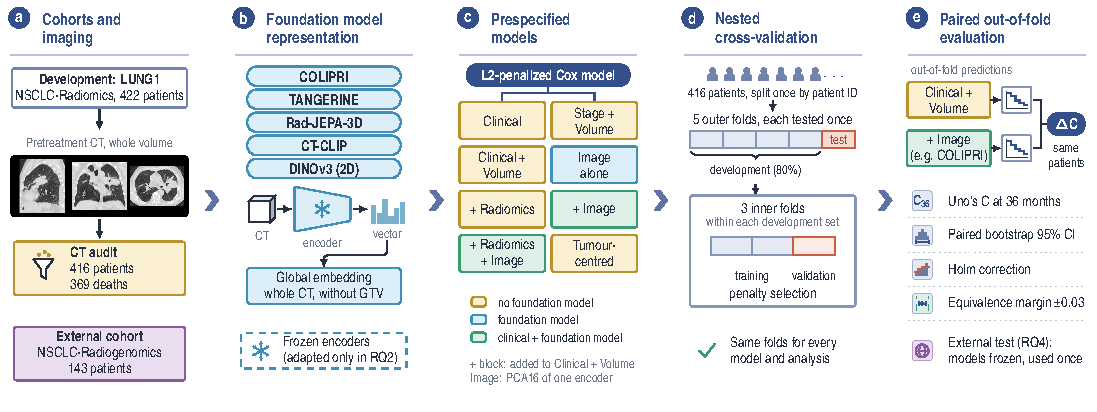
\includegraphics[width=\linewidth]{figures/study_overview.pdf}
\caption{Study design and analysis workflow. (a) LUNG1 provided all development data: after the CT audit, 416 patients had a pretreatment CT, a primary-tumour segmentation (GTV) and overall survival. NSCLC-Radiogenomics was used only for external evaluation. (b) Five foundation models encoded the whole CT with their published preprocessing and without the GTV into one global embedding per patient; the encoders were frozen except in the RQ2 adaptation analyses. (c) The prespecified models: nested clinical models, each adding one block to \model{Clinical+Volume}, the parsimonious \model{Stage+Volume} comparator, each image representation alone and the tumour-centred comparators. In the frozen benchmark, each embedding was reduced to its first 16 principal components (PCA16; 32, PCA32, in a sensitivity analysis), which entered an L2-penalized Cox model. (d) Five outer folds, fixed by patient before any model was fitted, and three inner folds for penalty selection were shared by every model and analysis. (e) Models were compared in pairs on the same test patients, for example \model{Clinical+Volume} with and without COLIPRI, by Uno's C at 36 months with paired bootstrap intervals, Holm correction and equivalence testing. For RQ4, models refitted on all 416 LUNG1 patients were frozen and applied once to the external cohort (purple).}
\label{fig:overview}
\end{figure}

The study was designed so that the main comparisons differ in the predictor being evaluated, while the evaluation protocol is held fixed. Every model, whether based on a whole-volume encoder, on tumour-centred features or on clinical covariates alone, was evaluated on the same patients, the same five outer folds, the same endpoint and horizon and the same metric, so that every comparison is paired at the patient level. Each foundation model was used with its published preprocessing and pooling (Section~\ref{sec:representations}). The clinical models were not treated as one more representation but as the reference against which the added value of each image representation was assessed (Section~\ref{sec:clinical}). In the frozen benchmark, the five foundations also shared the same head (Section~\ref{sec:partitioning}), so that differences between them reflect the representation together with its preprocessing and pooling. Within this fixed design, the four research questions RQ1-RQ4 in Section~\ref{sec:intro} differ in what they vary:
\begin{itemize}
\item RQ1 compares the representations under one frozen head, and asks whether an image representation adds to clinical information through a nested sequence of clinical models.
\item RQ2 changes what is trained, from a more flexible head to the encoder itself, and how many patients are available for training.
\item RQ3 changes what the encoder can see, by pooling tokens from different regions and by hiding the tumour inside the encoder, and asks which clinical variables the embeddings encode.
\item RQ4 changes the population: models developed on all LUNG1 patients were frozen and applied once to the external cohort.
\end{itemize}
Figure~\ref{fig:overview} gives an overview of the study as a single workflow shared by all four questions. Table~\ref{tab:design} lists the primary and sensitivity analyses that address each question within this workflow.

\tabDesign

The remainder of this section first describes the elements shared by all analyses: the cohorts and endpoint (Section~\ref{sec:cohorts}), the image representations and tumour-centred comparators (Section~\ref{sec:representations}), the clinical reference models (Section~\ref{sec:clinical}), and the data partitioning, model selection and frozen head (Section~\ref{sec:partitioning}). It then details the analyses for each research question (Section~\ref{sec:analyses}) and the performance measures and statistical methods (Section~\ref{sec:stats}).

\subsection{Cohorts}\label{sec:cohorts}
Cohorts used in this study are public collections of The Cancer Imaging Archive and provide, for each patient, a pretreatment CT, a primary-tumour segmentation and overall survival, so that every model can be computed on the same patients. LUNG1 was used for model development and internal evaluation, and NSCLC-Radiogenomics only for external evaluation. For each cohort, we describe why it was chosen and how the patients analysed were selected. We then compare the characteristics of the two cohorts and their implications for the analyses.

\paragraph{Development cohort.} LUNG1 contains pretreatment planning CT, a delineated primary gross tumour volume (GTV) and overall survival for 422 patients with NSCLC treated with radiotherapy, with or without chemotherapy, at a single institution.\cite{aerts2014,tciaLung1} It was chosen for three reasons. It is one of the largest public CT cohorts with survival outcomes and the cohort on which radiomic and deep prognostic models were first developed,\cite{aerts2014,hosny2018} so our results can be placed against published work. It provides the tumour segmentation required by the tumour-centred comparators and by the tumour-perturbation analyses. Finally, its follow-up is almost complete within the evaluation horizon, which keeps the concordance estimates close to what would be observed without censoring.

Survival in LUNG1 is measured from the start of treatment; death is the event, and patients without a recorded death are right-censored. The cohort was audited before any model was run. Clinical and imaging records were joined by patient identifier, and we required a positive survival time, a valid event code and a complete CT series with consistent geometry (no duplicated slice positions and no interslice gap larger than 1.5 times the median). Five of the 422 patients failed the CT audit, and one further patient had no primary-tumour segmentation, leaving 416 patients with 369 deaths (Figure~\ref{fig:overview}). All internal analyses used these 416 patients, so whole-volume and tumour-centred models were always compared on identical patients. Missing clinical covariates did not exclude a patient.

\paragraph{External cohort.} NSCLC-Radiogenomics includes 211 patients with NSCLC from two institutions in the United States, most of them treated with surgical resection, with preoperative CT, clinical data and, for 144 of them, a tumour segmentation.\cite{bakr2018,tciaRadiogenomics} It was chosen because it is one of the few public cohorts that combine CT, overall survival and tumour segmentations from institutions other than the LUNG1 provider, so that the same models, including the tumour-centred ones, can be applied without modification. We used only the patients with a segmentation, so that every model could be computed on the same patients and every external comparison is paired. The protocol for the external evaluation was fixed before any image of this cohort was processed. Survival was measured from the date of the CT used as input, because treatment dates were not available. Because a patient can have several CT series, for example reconstructions with different slice thickness, we used the series on which the segmentation had been drawn, so that image and mask were aligned. The same CT audit as in LUNG1 excluded one patient with missing slices, leaving 143 patients. Because the segmentations in the source collection carry inconsistent labels (``Heart'', ``Tissue'', ``Segmentation''), we confirmed that each one marked the tumour: its centre had to lie within 1 mm of an independent tumour seed point\cite{pai2024} and the mask had to overlap the lung field.

\paragraph{Cohort characteristics and their implications.} Table~\ref{tab:cohorts} and Figure~\ref{fig:km} describe the cohorts. They differ in almost every respect that affects a survival model, and these differences determine how the results should be read.

\begin{figure}[!htbp]
\centering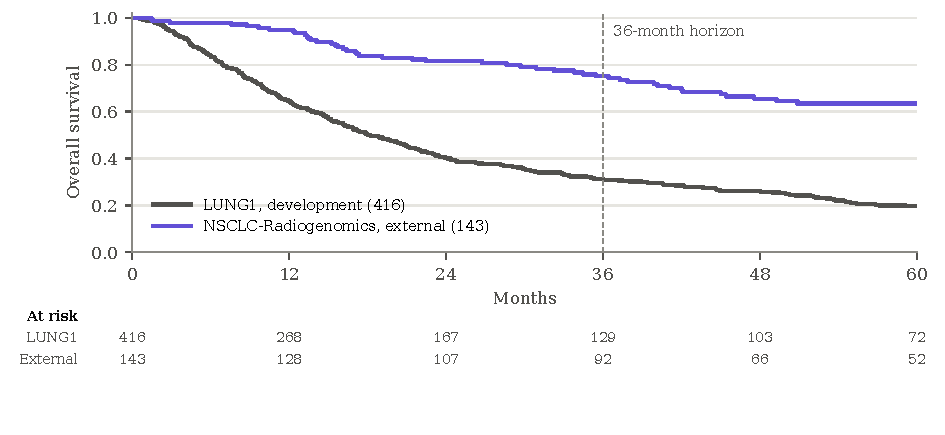
\includegraphics[width=\linewidth]{figures/cohort_km.pdf}
\caption{Kaplan--Meier estimates of overall survival in the development cohort (LUNG1, from the start of treatment) and in the external cohort (NSCLC-Radiogenomics, 143 patients with a tumour segmentation, from the date of the input CT). The dashed vertical line marks the 36-month horizon of the primary metric.}
\label{fig:km}
\end{figure}

% Generated by scripts/build_cohort_artifacts.py from data/derived/; do not edit by hand.
\begin{table}[!htbp]
\centering\footnotesize
\caption{Characteristics of the development and external cohorts. Values are $n$ (\%) unless stated otherwise. Survival in LUNG1 is measured from the start of treatment and in NSCLC-Radiogenomics from the date of the input CT. LUNG1 records clinical TNM and NSCLC-Radiogenomics pathological TNM; both were mapped to the same categories (Section~\ref{sec:clinical}). IQR, interquartile range; GTV, gross tumour volume.
$^{a}$Reverse Kaplan--Meier estimate.
$^{b}$From the primary-tumour segmentation.
$^{c}$Seventh-edition AJCC stage; in NSCLC-Radiogenomics, the four stage IV (M1) patients are counted as IIIb, the highest LUNG1 category. Legacy LUNG1 codes T5 ($n=2$) and N4 ($n=3$) are counted as T4 and N3.}
\label{tab:cohorts}
\begin{tabular}{@{}lrr@{}}
\toprule
 & LUNG1 & NSCLC-Radiogenomics \\
 & development & external \\
\midrule
Patients & 416 & 143 \\
Deaths, overall & 369 (89) & 50 (35) \\
Deaths by 36 months & 286 (69) & 33 (23) \\
Censored before 36 months & 1 (0) & 18 (13) \\
Median follow-up, months$^{a}$ & 116 & 62 \\
Median overall survival, months & 18.0 & not reached \\
36-month survival, \% (95\% CI) & 31 (27--36) & 75 (67--82) \\
Age, years, median (IQR) & 69 (62--76) & 69 (64--76) \\
\quad Age missing & 22 & 0 \\
Male sex & 287 (69) & 107 (75) \\
\multicolumn{3}{@{}l}{T category}\\
\quad T1 & 93 (22) & 74 (52) \\
\quad T2 & 155 (37) & 48 (34) \\
\quad T3 & 51 (12) & 16 (11) \\
\quad T4 & 117 (28) & 5 (3) \\
\multicolumn{3}{@{}l}{N category}\\
\quad N0 & 168 (40) & 115 (80) \\
\quad N1 & 22 (5) & 11 (8) \\
\quad N2 & 141 (34) & 17 (12) \\
\quad N3 & 85 (20) & 0 (0) \\
\multicolumn{3}{@{}l}{Overall stage$^{c}$}\\
\quad I & 93 (22) & 93 (65) \\
\quad II & 40 (10) & 25 (17) \\
\quad IIIa & 111 (27) & 20 (14) \\
\quad IIIb & 171 (41) & 5 (3) \\
\quad TNM or stage missing & 1 (0) & 0 (0) \\
\multicolumn{3}{@{}l}{Histology}\\
\quad Adenocarcinoma & 51 (12) & 112 (78) \\
\quad Squamous cell carcinoma & 151 (36) & 28 (20) \\
\quad Large cell carcinoma & 114 (27) & 0 (0) \\
\quad NSCLC, not otherwise specified & 61 (15) & 3 (2) \\
\quad Histology missing & 39 (9) & 0 (0) \\
GTV volume, cm$^3$, median (IQR)$^{b}$ & 39.1 (10.4--102.0) & 8.1 (3.5--24.2) \\
\bottomrule
\end{tabular}
\end{table}


LUNG1 is a cohort of advanced disease: 68\% of patients had stage III disease, median survival was 18 months, and 69\% had died by 36 months, with only one patient censored before that time. Two consequences follow. First, the event rate is high rather than low: the concordance at 36 months is computed almost entirely among patients who died, and measures how well a model orders the times to death rather than separating a minority of events from many survivors. Second, overall stage varies little, so stage-based models are expected to discriminate only modestly in this cohort. Prognostic models developed on or applied to LUNG1 have reported concordance of about 0.58 to 0.65,\cite{aerts2014} which sets a realistic expectation: differences between models of a few hundredths of a concordance unit are the scale of interest, and with 416 patients only differences of about 0.05 can be detected with adequate power (Section~\ref{sec:stats}).

The external cohort is the opposite: 65\% of patients had stage I disease, 78\% had adenocarcinoma, the median GTV was about one fifth of that in LUNG1, and 75\% were alive at 36 months. Only 33 deaths occurred by 36 months. Treatment, case mix, TNM source (clinical in LUNG1, pathological in NSCLC-Radiogenomics), time origin and scanners (mainly Siemens and 3-mm slices in LUNG1; mainly GE and 1.25-mm slices externally) all differ. The external evaluation is therefore a test of transport under population and acquisition shift, not a replication. We expected three things before applying any model: wide intervals, with differences between models of less than about 0.08 not detectable; poor absolute calibration, because the baseline hazard estimated in LUNG1 is far higher than the external one; and, because many deaths in an early-stage surgical population may not be cancer-related, image models that capture age and general anatomy could transport at least as well as \model{Stage+Volume}, which varies little in this population. The last expectation was recorded as a hypothesis in the external protocol.

\paragraph{Endpoint.} The endpoint was overall survival, and the prediction horizon was 36 months. The horizon was fixed before the results. It lies within the follow-up of nearly all LUNG1 patients and of most external patients (median follow-up 116 and 62 months, respectively; Table~\ref{tab:cohorts}), and it uses the continuous survival time rather than a binary two-year status, as in several earlier studies.\cite{hosny2018,aerts2025tib}

\FloatBarrier
\subsection{Image representations}\label{sec:representations}
We compared eight image representations: five foundation-model encoders that see the whole CT and three tumour-centred comparators that use the segmented tumour. Table~\ref{tab:representations} gives, for each one, its pretraining, its input preprocessing, how its global vector is obtained and the dimension of that vector. The four whole-volume CT encoders (COLIPRI, TANGERINE, Rad-JEPA-3D and CT-CLIP) were chosen because they have public weights, accept a complete three-dimensional CT volume and were pretrained with different objectives, so that the comparison spans the main pretraining paradigms. DINOv3, trained only on natural images, was added as a reference for what a general-purpose encoder achieves without any medical pretraining. The tumour-centred comparators represent the established approaches on LUNG1: handcrafted radiomics of the segmented tumour, a lesion-level foundation model (Pai)\cite{pai2024} and a supervised deep network trained for two-year survival (Hosny).\cite{hosny2018}

\tabRepresentations

\paragraph{Preprocessing.} Every pipeline started from the same audited CT series, loaded as a three-dimensional volume in Hounsfield units. Each encoder then received its published preprocessing: orientation, resampling, intensity window and crop or padding were those of the original model (Table~\ref{tab:representations}). We did not impose a common preprocessing, because an encoder is only meaningful with the input distribution on which it was pretrained. The price is that the encoders see different fields of view and resolutions, so differences between pipelines combine pretraining, preprocessing and pooling, and cannot be attributed to the pretraining objective alone. The whole-volume encoders and DINOv3 received the whole CT without any segmentation. DINOv3, a two-dimensional encoder, embedded each axial slice, and the slice embeddings were averaged.

\paragraph{Global and token representations.} For each encoder we used the global vector defined by its authors: a learned attention pool for COLIPRI, the class token concatenated with the mean patch token for TANGERINE, the mean of final tokens for Rad-JEPA-3D, the projected temporal mean for CT-CLIP and the slice-averaged class token for DINOv3. Using the authors' pooling avoids designing a new pooling rule that might favour one encoder. These vectors were extracted once, without survival labels, and were the input of the frozen benchmark and of the multilayer perceptron. The survival query adapter and the regional pooling analysis used the final spatial tokens instead, averaged onto a grid of at most eight cells per axis; the native-token masking analysis worked on each encoder's native token grid (Section~\ref{sec:perturbation}).

\paragraph{Tumour-centred comparators.} The radiomic model used 107 PyRadiomics original-image features (shape, first-order and texture) from the GTV on a 1-mm isotropic grid. This is a practical baseline in the spirit of the LUNG1 radiomic signature, not a reproduction of it.\cite{aerts2014} The Pai lesion encoder and the Hosny network received a 50-mm cubic patch at 1-mm spacing centred on the GTV centroid, with their published intensity normalization; our centroids agreed with the seed points distributed with the Pai model (median distance 0.16 mm). The Hosny network was reimplemented from the published weights, and it reproduced the published outputs on the authors' example inputs. LUNG1 was not used to train it, so its published two-year risk score was also evaluated without any refitting (\emph{Hosny zero-shot}).

These comparators use the tumour location, which the whole-volume encoders do not receive. This asymmetry favours the tumour-centred comparators and is kept deliberately: it compares each approach in the form in which it would be used.

\subsection{Clinical reference models}\label{sec:clinical}
The clinically relevant question is not whether an image representation predicts survival on its own, but whether it adds prognostic information to what is already known about the patient. To answer it, we defined a set of clinical reference models (Table~\ref{tab:clinical}), built as a nested sequence in which each model adds one block to the previous one. Each model is named after its content, so that every comparison reads as the block being added.

\tabClinical

The covariates of the \model{Clinical} model were restricted to variables that also exist in NSCLC-Radiogenomics, so that the same models could be evaluated externally. Metastasis category was excluded because 411 of the 416 LUNG1 patients were M0. \model{Stage+Volume}, the two established prognostic factors in this population,\cite{goldstraw2016,bradley2002} was added as a parsimonious comparator outside the nested sequence, because a model with many weak covariates can be a weaker baseline than one with few strong ones.

Age was median-imputed within each training set with a missingness indicator, and missing categorical values were coded as a separate category. Overall stage was coded as I, II, IIIa or IIIb, T as T1--T4 and N as N0--N3. The legacy LUNG1 codes T5 ($n=2$) and N4 ($n=3$), whose meaning the source collection describes as uncertain, were merged into T4 and N3. In NSCLC-Radiogenomics, pathological TNM was mapped onto the same categories, with stage derived from TNM according to the seventh edition of the AJCC staging system and the four stage IV patients assigned to IIIb, the highest LUNG1 category.

When an image or radiomic block was combined with clinical covariates, the clinical block and the image or radiomic block received separate L2 penalties, each chosen from $\{0.01, 0.1, 1\}$ by inner cross-validation. This prevents the few clinical covariates from being shrunk as strongly as the many image features, which would otherwise make the image block appear to replace rather than add to the clinical information.

\subsection{Data partitioning and model selection}\label{sec:partitioning}
Figure~\ref{fig:partitioning} shows how patients were used. The 416 LUNG1 patients were divided once into five outer folds, stratified by event status and by early (I--II) versus late (IIIa--IIIb) stage, and the assignment was locked by patient identifier before any model was fitted. Within each outer development set (approximately 332 patients), three event-stratified inner folds were also fixed. The same outer and inner folds were used by every model, encoder and analysis, so that all internal comparisons are paired and every hyperparameter was selected on the same patients.

% Patient use per outer fold in each analysis. Included from sections/methods.tex.
% Horizontal scale: 1 patient = 0.02 cm (416 patients = 8.3 cm).
\begin{figure}[!htbp]
\centering
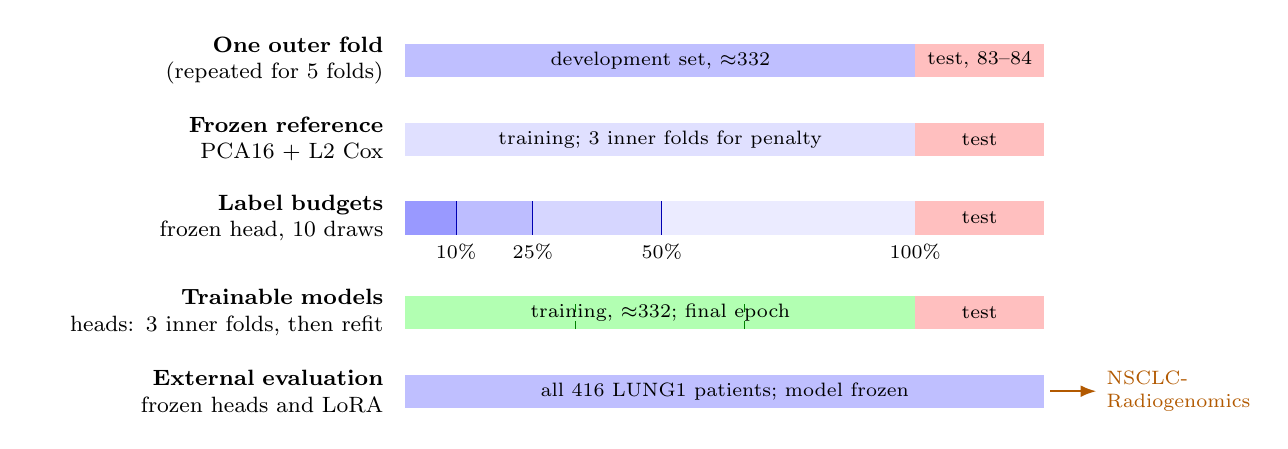
\begin{tikzpicture}[font=\footnotesize, x=0.0195cm, y=1cm,
  seg/.style={draw=white, line width=0.6pt},
  lab/.style={anchor=east, align=right, text width=4.4cm},
  inb/.style={font=\scriptsize, align=center}]
\def\rowh{0.42}
\newcommand{\pbar}[5]{% y, from, to, colour, label
  \fill[#4] (#2,#1) rectangle (#3,#1+\rowh);
  \node[inb] at ({(#2+#3)/2},#1+\rowh/2) {#5};}
% Row 1: outer fold
\node[lab] at (-8,0.21) {\textbf{One outer fold}\\(repeated for 5 folds)};
\pbar{0}{0}{332}{blue!25}{development set, $\approx$332}
\pbar{0}{332}{416}{red!25}{test, 83--84}
% Row 2: frozen reference
\node[lab] at (-8,-0.79) {\textbf{Frozen reference}\\PCA16 + L2 Cox};
\pbar{-1}{0}{332}{blue!12}{training; 3 inner folds for penalty}
\pbar{-1}{332}{416}{red!25}{test}
% Row 3: label budgets (nested)
\node[lab] at (-8,-1.79) {\textbf{Label budgets}\\frozen head, 10 draws};
\fill[blue!8] (0,-2) rectangle (332,-2+\rowh);
\fill[blue!16] (0,-2) rectangle (167,-2+\rowh);
\fill[blue!26] (0,-2) rectangle (83,-2+\rowh);
\fill[blue!40] (0,-2) rectangle (33,-2+\rowh);
\foreach \x/\t in {33/10\%, 83/25\%, 167/50\%, 332/100\%}
  \node[font=\scriptsize, anchor=north] at (\x,-2) {\t};
\foreach \x in {33,83,167} \draw[blue!70!black] (\x,-2) -- (\x,-2+\rowh);
\pbar{-2}{332}{416}{red!25}{test}
% Row 4: nested selection and refit (all trainable models)
\node[lab] at (-8,-2.99) {\textbf{Trainable models}\\heads: 3 inner folds, then refit};
\pbar{-3.2}{0}{332}{green!30}{training, $\approx$332; final epoch}
\foreach \x in {111,221} \draw[green!50!black, dashed] (\x,-3.2) -- (\x,-3.2+\rowh);
\pbar{-3.2}{332}{416}{red!25}{test}
% Row 5: external evaluation
\node[lab] at (-8,-3.99) {\textbf{External evaluation}\\frozen heads and LoRA};
\pbar{-4.2}{0}{416}{blue!25}{all 416 LUNG1 patients; model frozen}
\draw[-{Latex[length=2mm]}, thick, orange!70!black] (420,-4.2+\rowh/2) -- (450,-4.2+\rowh/2)
  node[right, align=left, font=\scriptsize] {NSCLC-\\Radiogenomics};
\end{tikzpicture}
\caption{Use of LUNG1 patients in each analysis. The first four rows show one of the five fixed outer folds, which were identical across analyses; test patients (red) were never used for fitting, model selection or hyperparameter choice. In the label-budget analysis, smaller training subsets (ten draws below full budget) are contained in larger ones, and Uno C censoring weights were estimated from the full development set at every budget. Frozen and trainable heads were selected on the same three inner folds (dashed) and then retrained on the whole development set; LoRA and partial fine-tuning used a fixed configuration on the whole development set.}
\label{fig:partitioning}
\end{figure}


\paragraph{Frozen head.} The frozen head standardized the global vector, reduced it to 16 principal components (PCA16) and fitted an L2-regularized Cox model, with the penalty selected by three-fold inner cross-validation. The reduction to a fixed number of components serves two purposes. It gives every representation the same head capacity although their dimensions range from 107 to 4,096, so that differences reflect the information in the representation rather than the number of parameters fitted; and it keeps the number of parameters well below the number of events (about 295 deaths per development set at full budget, about 29 at the smallest budget). The number of components was not tuned per encoder, because selecting it on the same small cohort would add a second source of optimism. The original protocol used 16 components, and the 32-component head (PCA32) is reported as a sensitivity analysis. The radiomic and \model{Stage+Volume} baselines used all their covariates without dimensionality reduction.

\subsection{Analyses by research question}\label{sec:analyses}
This section describes the analyses that address each research question, in the order of Table~\ref{tab:design}. All of them use the cohorts, representations, clinical reference models and folds described above. 

\subsubsection{RQ1: frozen benchmark and clinical increment}\label{sec:frozen}
RQ1 asks two questions about the representations as they are, without any training of the encoder. The first is how much survival information each representation provides compared with the others and with established image-based predictors, when all of them are given the same head. The second is whether this information adds to what the clinical covariates and tumour volume already provide, which is the comparison that matters for clinical use. Two analyses address them, in the same outer folds: the frozen benchmark and the clinical increment analysis.

The \emph{frozen benchmark} fitted the frozen head to each representation in every outer fold and compared the representations with each other and with \model{Stage+Volume}, the radiomic model and the tumour-centred comparators. The highest mean-fold concordance reached by any frozen model on LUNG1 was taken as an empirical reference for the information accessible without training the encoder.

The \emph{clinical increment analysis} fitted the nested clinical models of Table~\ref{tab:clinical} in the same folds. Its five prespecified primary contrasts, which formed one Holm family, asked whether tumour volume adds to clinical covariates (\model{Clinical+Volume} vs \model{Clinical}), whether radiomics adds to them (\model{Clinical+Volume+Radiomics} vs \model{Clinical+Volume}), whether COLIPRI adds to them (\model{Clinical+Volume+COLIPRI} vs \model{Clinical+Volume}), whether radiomics adds to COLIPRI (\model{Clinical+Volume+Radiomics+COLIPRI} vs \model{Clinical+Volume+COLIPRI}) and whether COLIPRI adds to radiomics (\model{Clinical+Volume+Radiomics+COLIPRI} vs \model{Clinical+Volume+Radiomics}). COLIPRI was designated in advance as the image block of the full model, because it had the highest frozen discrimination in earlier analyses; TANGERINE was used as a sensitivity analysis. Secondary families repeated the image-over-clinical contrast for every encoder and the reverse contrast, clinical information over the image representation alone. The Pai and Hosny representations entered the same sequence in place of the whole-volume encoder, as the image block of \model{Clinical+Volume+Image}, so that their increment over clinical information was assessed in the same way.

\subsubsection{RQ2: trainable heads, encoder adaptation and label budget}\label{sec:selected}
RQ2 asks whether a more flexible head, or updating the encoder itself, improves on the frozen head. Table~\ref{tab:trainable} describes the four trainable models: two heads that keep the encoder frozen and two methods that update its final block, which is the last transformer block for TANGERINE, COLIPRI and DINOv3 and the last hybrid Mamba block for Rad-JEPA-3D. In CT-CLIP, the vector quantizer stops gradients between the exported visual embedding and the encoder blocks, so LoRA and partial fine-tuning were applied to its final visual projection, giving it a different trainable capacity. The Breslow baseline hazard was always estimated on the training patients.

\tabTrainable

The four trainable models of Table~\ref{tab:trainable} were evaluated in two analyses, which differ in how much is trained: in the \emph{trainable-head comparison} only the two heads are trained, with the encoder frozen; in the \emph{encoder-adaptation analysis} LoRA and partial fine-tuning also update the final block of the encoder. A third analysis, the \emph{label-budget analysis}, does not train any new model: it refits the frozen head on fewer training patients, to test whether the foundation models need fewer labelled patients than the baselines. All three use the same folds, endpoint and metric as the frozen benchmark.

\paragraph{Trainable-head comparison.} The multilayer perceptron, and the survival query adapter, which attends to the frozen spatial tokens with four learned queries, were selected with the same nested procedure as the frozen head. Within each outer development set, the number of training epochs was selected by three-fold inner cross-validation: each candidate was trained on two inner folds (approximately 221 patients) and scored on the third (approximately 111 patients), and the epoch count with the highest validation concordance averaged over the three inner folds was selected, with ties resolved towards fewer epochs. The selected head was then retrained on the whole development set and evaluated once on the test fold at its final epoch.

\paragraph{Encoder adaptation.} LoRA\cite{hu2021} and partial fine-tuning of the final block used one fixed configuration for all five encoders: a learning rate of $10^{-3}$ for LoRA and $10^{-4}$ for partial fine-tuning, each for 20 epochs, trained on the whole development set and evaluated at the final epoch. Training stability was examined post hoc from the training loss and the spread of predicted risks; the configuration was not changed for any encoder. All trainable models were thus trained on the same development patients and tested on the same patients as the frozen head.

\paragraph{Label-budget analysis.} To measure how discrimination depends on the number of labelled patients, the frozen heads and the \model{Stage+Volume} and radiomic baselines were refitted on subsets of 10\%, 25\%, 50\% and 100\% of the training patients of each outer fold and evaluated on the unchanged test folds. Penalty selection used only the patients in the subset. With a small budget, the result depends on which patients happen to be drawn: at 10\%, a subset contains about 33 patients. Each subset below 100\% was therefore drawn ten times, and the concordance at each budget is the mean over the ten draws. Each draw was nested (its 10\% subset contained in its 25\% subset, and that in its 50\% subset) and stratified by event status and, at 25\% and 50\%, by early versus late stage. All models were fitted on the same draws, so that the comparisons at each budget remain paired. The censoring weights of the concordance were estimated once from the full development set, so that differences between budgets reflect the fitted models rather than the evaluation weights. The number of components was fixed across budgets to keep head capacity constant. 

\subsubsection{RQ3: tumour dependence}\label{sec:perturbation}
RQ3 asks how sensitive the representations and their survival predictions are to the tumour, that is, whether the survival information in the whole-volume representations comes from the primary tumour or from the rest of the scan. No single intervention can remove the tumour without also changing something else, so four analyses approach the question from complementary directions. The \emph{regional pooling analysis} asks where in the scan the useful tokens lie; the \emph{native-token masking analysis} hides the tumour inside the encoder and refits the head; the \emph{fixed-head masking analysis} applies the original head to the masked embeddings; and \emph{clinical-variable probing} describes which clinical variables the embeddings encode, with and without the tumour. Figure~\ref{fig:rq3design} summarizes the input, encoder, representation, survival model or probe and outcome measure of each.

% RQ3 design: the four tumour-dependence analyses. Included from sections/methods.tex.
% Source: figures/figure4/rq3_design_fig.tex (build commands in its header).
\begin{figure}[!htbp]
\centering
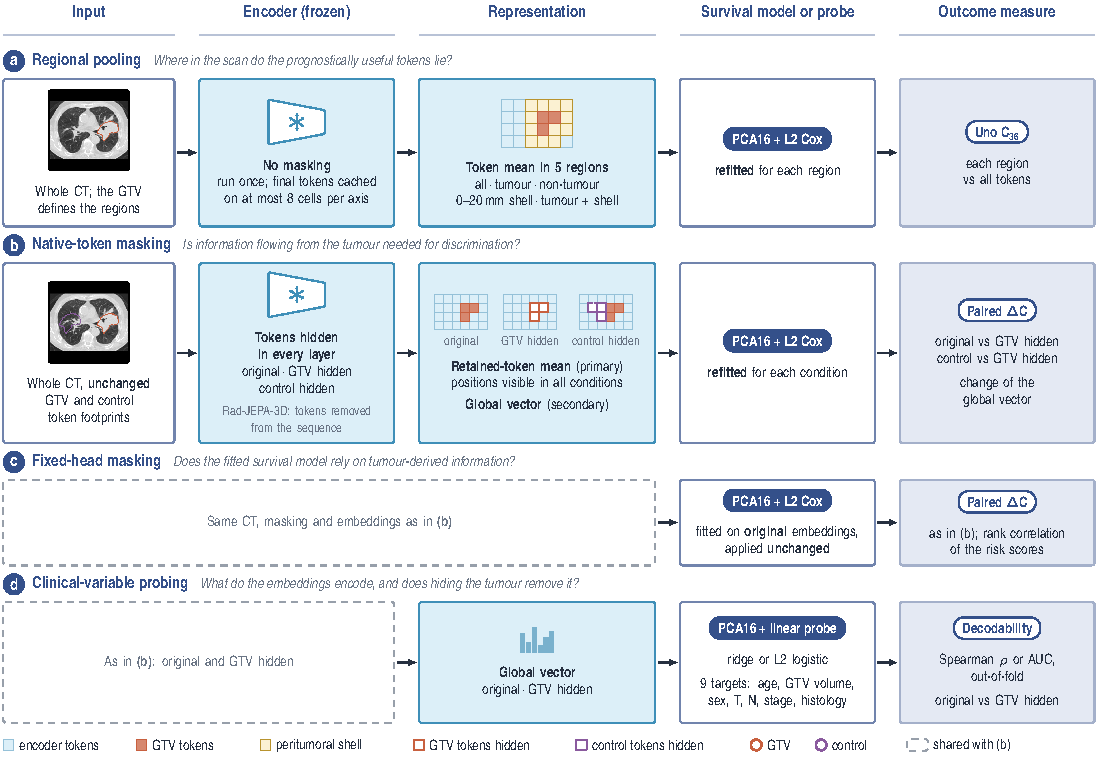
\includegraphics[width=\linewidth]{figures/rq3_design.pdf}
\caption{Design of the four tumour-dependence analyses (RQ3). Each row shows the input, the frozen encoder, the representation, the survival model or probe and the outcome measure. All survival models and probes were fitted on the development folds, with penalties selected by three-fold inner cross-validation, and evaluated on the same five outer test folds. (a) Regional pooling pools the cached final tokens of the unmasked encoder over regions defined by the primary tumour (GTV). (b) Native-token masking leaves the CT unchanged and hides, in every layer of the encoder, the native tokens that contain a GTV voxel, or the same number of tokens around the GTV shape translated within the same axial level (control). Each CT is encoded three times: original, GTV hidden and control hidden. In all three, the primary representation averages the tokens at the same positions, outside both the GTV and the control region, so the conditions differ only in what these tokens received from the hidden region inside the encoder. (c) Fixed-head masking uses the embeddings of (b) but does not refit the survival model. (d) Probing decodes clinical variables from the global vector, with and without the tumour hidden. The CT slice (LUNG1-001) and the control outline are illustrative; grid icons show a single axial level, whereas pooling and masking were applied to the three-dimensional token grid.}
\label{fig:rq3design}
\end{figure}


\paragraph{Regional pooling analysis.} The cached final tokens of each encoder were pooled over five regions defined from the GTV, without re-encoding the CT: all tokens; tumour tokens, weighted by the fraction of each token occupied by the GTV; non-tumour tokens with no GTV overlap; a peritumoral shell from 0 to 20 mm around the GTV; and the union of tumour and shell (Figure~\ref{fig:rq3design}a). Each pooled vector was passed to the frozen head. Because the tokens had already exchanged information inside the encoder, the non-tumour pool still contains information that came from the tumour; this analysis therefore asks \emph{where} useful token positions lie, not whether the tumour is needed.

\paragraph{Native-token masking analysis.} To remove the tumour's contribution inside the encoder, every native token containing a GTV voxel was hidden in every layer of the frozen encoder, while the CT input was left unchanged (Figure~\ref{fig:rq3design}b). In attention-based encoders, the keys of the hidden tokens were masked in every attention layer, and their outputs were excluded from every pooling; for a transformer this is equivalent to removing the tokens while keeping the positions of the others. In CT-CLIP, attention is not the only route between tokens: its blocks also mix neighbouring tokens through depthwise convolutions, so the hidden tokens were additionally set to zero at the input of every such convolution. Rad-JEPA-3D is a state-space hybrid without attention to mask, so the hidden tokens were removed from the sequence through the encoder's own context-index mechanism used during its pretraining. A leakage test replaced the hidden voxels with random noise: with masking on, the retained tokens and global vectors did not change for any encoder.

A loss of discrimination after hiding the GTV would not, on its own, show that the tumour matters, because hiding any region of the scan changes the representation, even a region with no prognostic information. To separate the effect of hiding the tumour from the effect of hiding tokens as such, we added a control condition, which hid the same number of tokens around the GTV shape translated to another position at the same axial level. The contrast between the control-hidden and tumour-hidden conditions therefore isolates the contribution of the tumour; a valid control was available for 403 patients. The primary pooling was the mean of the tokens visible in every condition, so that the original, tumour-hidden and control-hidden conditions were pooled over identical positions and differed only in whether those tokens could receive information from the hidden region. The encoder's own global vector was a secondary representation. Each condition was passed to a frozen head refitted for that condition. The analysis also measured how much the global vector changed relative to the original, to separate a change in the representation from a change in discrimination.

\paragraph{Fixed-head masking analysis.} Refitting the head on masked embeddings lets it adapt to the perturbation. In this analysis, the frozen head fitted on the original embeddings was applied unchanged to the tumour-hidden and control-hidden embeddings, which asks whether the fitted model relies on tumour-derived information.

\paragraph{Clinical-variable probing.} To describe what the embeddings encode, we tested how well clinical variables could be decoded from the global vectors, in the original and tumour-hidden conditions. The targets were age and log GTV volume (Spearman correlation) and male sex, T3--T4, any nodal involvement, N2--N3, stage III, squamous histology and adenocarcinoma (area under the ROC curve). Probes were ridge or L2-regularized logistic regressions on PCA16, with the penalty chosen by three-fold inner cross-validation; they were evaluated on the pooled out-of-fold predictions of the same outer folds, and all components were also used as a sensitivity analysis. Decodability shows that a variable is encoded; it does not show that the survival prediction uses it.

\subsubsection{RQ4: external evaluation}\label{sec:external}
RQ4 asks whether discrimination, incremental clinical value and calibration transfer to an external cohort, that is, whether models developed on LUNG1 keep their performance when applied, without any change, to patients from other institutions. Two analyses address it: the \emph{external evaluation} applies the models of RQ1 to NSCLC-Radiogenomics; the \emph{external LoRA analysis}, added as exploratory, does the same for the adapted encoders of RQ2.

For the \emph{external evaluation}, 22 models were refitted on all 416 LUNG1 patients with the same selection procedure used internally (penalties by three-fold cross-validation on the 416 patients; imputation, scaling and dimensionality reduction fitted on them): the nested clinical models, \model{Stage+Volume}, the radiomic model, the frozen head of every representation, and the Hosny zero-shot score. The external CTs received exactly the same preprocessing as LUNG1, without harmonization of intensities, kernels or slice thickness, because the aim was to test the models as they would be applied to a new hospital. The only correction was a decoding one: out-of-field padding stored below $-1024$ HU by some scanners was set to $-1024$ HU, the minimum value in every LUNG1 scan. No external recalibration was applied.

The four primary contrasts, fixed in advance, were COLIPRI vs \model{Stage+Volume}, \model{Clinical+Volume+COLIPRI} vs \model{Clinical+Volume}, COLIPRI vs the Pai lesion encoder, and COLIPRI vs Hosny zero-shot. Secondary outcomes were the concordance of all other models, the concordance at 60 months, the calibration of absolute risk and the Spearman correlation between internal and external concordance across models, which asks whether the ranking of pipelines transports. The trainable heads and the adaptation models were not carried over to the original external evaluation, because none of them had exceeded the frozen head internally at the time the external protocol was fixed.

In the \emph{external LoRA analysis}, LoRA models for all five encoders were trained on all 416 LUNG1 patients with the fixed adaptation configuration, frozen in the same way and evaluated on the external cohort, with paired comparisons against the corresponding frozen heads. This analysis was added after the external cohort had been examined in the original evaluation and uses a configuration chosen on LUNG1 test folds.

\subsection{Performance measures and statistical analysis}\label{sec:stats}
\paragraph{Discrimination.} The primary measure was Uno's concordance index truncated at 36 months (Uno C),\cite{uno2011} which weights comparable pairs by the inverse probability of censoring and is therefore less dependent on the censoring distribution than Harrell's index. For test patients with observed time $T_i$, event indicator $\delta_i$ and predicted risk $\eta_i$,
\begin{equation}\label{eq:unoc}
C_\tau=\frac{\sum_{i}\sum_{j}\delta_i\,\hat{G}(T_i)^{-2}\,\mathbf{1}(T_i<T_j,\;T_i\le\tau)\left[\mathbf{1}(\eta_i>\eta_j)+\frac{1}{2}\mathbf{1}(\eta_i=\eta_j)\right]}{\sum_{i}\sum_{j}\delta_i\,\hat{G}(T_i)^{-2}\,\mathbf{1}(T_i<T_j,\;T_i\le\tau)},
\end{equation}
where $\hat{G}$ is the Kaplan--Meier estimate of the censoring survival function, $\tau=36$ months, and ties in predicted risk count as one half. Internally, the censoring distribution was estimated from the development patients of each outer fold, and the primary estimate was the mean of the five test-fold values. Externally, the censoring distribution was estimated from the relevant external population.

\paragraph{Calibration.} Absolute risk was assessed externally by comparing observed mortality at 36 months (Kaplan--Meier) with mean predicted mortality, using the LUNG1 Breslow baseline hazard, and by the calibration slope, the coefficient of a Cox regression of the outcome on the linear predictor.\cite{vancalster2019,austin2020}

\paragraph{Uncertainty and tests.} Uncertainty was estimated with paired patient bootstrap resampling. Internally, test patients were resampled within each fixed fold and the fold estimates were averaged, with the same resamples shared by all models compared; externally, patients were resampled from the external population. We used 1,000 resamples for the clinical increment and trainable-model comparisons, 300 for the masking analyses and 2,000 for the external evaluation. Intervals are 95\% percentile intervals, and $p$ values come from a two-sided Wald test with the bootstrap standard error. These intervals condition on the fitted models and on the fold assignment; they do not include the variability from refitting the models on different patients.

Because most analyses involved several comparisons, $p$ values were adjusted with the Holm method within families of comparisons fixed in advance. Each of the following formed one family: the five primary contrasts of the clinical increment analysis (Section~\ref{sec:frozen}); each of its secondary contrasts, repeated across encoders (image over \model{Clinical+Volume}, clinical over image, radiomics over image, and image vs radiomics); the 22 comparisons of a trainable model with the frozen head of the same encoder (seven multilayer perceptron, five survival query adapter, five LoRA and five partial fine-tuning models; Section~\ref{sec:selected}); the four primary contrasts of the external evaluation (Section~\ref{sec:external}); and the comparisons of each external model with chance. Intervals for the masking and probing analyses (Section~\ref{sec:perturbation}), the label-budget analysis (Section~\ref{sec:selected}) and the external LoRA analysis (Section~\ref{sec:external}) are reported without multiplicity adjustment, and no hypothesis test is attached to the preliminary fixed-epoch analysis. A nonsignificant difference was not interpreted as absence of a difference: equivalence was declared when the 90\% bootstrap interval of a difference lay within a margin of $\pm0.03$ Uno C, fixed in advance (two one-sided tests), and for every contrast we report the minimum detectable difference, $(z_{0.975}+z_{0.80})$ times the bootstrap standard error. Contrasts smaller than this value are reported as inconclusive rather than negative.

\subsection{Implementation}
Survival models were implemented in Python with PyTorch Lightning for the neural models and lifelines for the linear Cox models; radiomic features were extracted with PyRadiomics 3.0.1. Neural models optimized the Cox partial likelihood with Efron ties, with the risk-set computations in single precision. Internal training used BF16 mixed precision on NVIDIA A100 GPUs; the external LoRA models were trained with FP16 mixed precision on an NVIDIA V100 for COLIPRI and TANGERINE and with BF16 on an A100 for the other three encoders. Each run stored a protocol file with the hashes of the cohort, the fold assignment, the encoder checkpoint and the cached inputs.
\gap{Add the code repository URL and the full list of software versions after the release inventory is verified.}

\section{Results}\label{sec:results}
The results are reported by research question, in the order set out in Section~\ref{sec:design}: RQ1 in Section~\ref{sec:res-rq1}, RQ2 in Section~\ref{sec:res-adaptation}, RQ3 in Section~\ref{sec:res-rq3} and RQ4 in Section~\ref{sec:res-rq4}. Each subsection is titled by its question and reports the primary analysis before the sensitivity analyses.

In summary, frozen COLIPRI had the highest discrimination on LUNG1 and exceeded \model{Stage+Volume} and radiomics in point estimate, by about 0.03 with 16 components and 0.045 with 32, but none of these differences was statistically significant after Holm correction, and no encoder significantly added to the clinical covariates (RQ1). Neither trainable heads nor encoder adaptation improved on the frozen linear head, and the encoders showed no advantage in label efficiency (RQ2). Only COLIPRI was sensitive to the tumour, and hiding the tumour inside any encoder lowered discrimination by at most 0.013 (RQ3). Externally, risk ordering by the stronger encoders transported, whereas their incremental clinical value remained unresolved and their absolute risks were miscalibrated (RQ4).

All internal estimates are mean-fold Uno C at 36 months on the 416 LUNG1 patients. Intervals are 95\% paired bootstrap intervals conditional on the fitted models, $p$ values are Holm-adjusted within the families of Section~\ref{sec:stats}, and ``equivalent'' means that the 90\% interval of a difference lay within the $\pm0.03$ margin.

\subsection{RQ1: How much prognostic information is accessible from frozen foundation-model representations, relative to clinical, radiomic and tumour-centred models?}\label{sec:res-rq1}

Frozen discrimination was modest for every model (Figure~\ref{fig:rq1}a). COLIPRI was the highest, at 0.617 (0.582 to 0.652), followed by TANGERINE (0.599), DINOv3 (0.575), Rad-JEPA-3D (0.539) and CT-CLIP (0.530). The clinical covariates alone were close to chance (\model{Clinical}, 0.529; 0.493 to 0.565), and \model{Stage+Volume} reached 0.588. The tumour-centred comparators ranged from 0.555 (Pai lesion encoder) to 0.591 (GTV radiomics). With the 32-component head (PCA32), a sensitivity analysis of head capacity added after the PCA16 comparisons (open markers in Figure~\ref{fig:rq1}a), COLIPRI reached 0.634 (0.600 to 0.669), followed by TANGERINE (0.607), DINOv3 (0.560), Rad-JEPA-3D (0.559) and CT-CLIP (0.527). Each encoder changed by $-0.014$ to $+0.020$ relative to PCA16, none significantly (Table~\ref{tab:trainable_results}), and the two leading encoders were the same with both heads.
\begin{figure}[!t]
\centering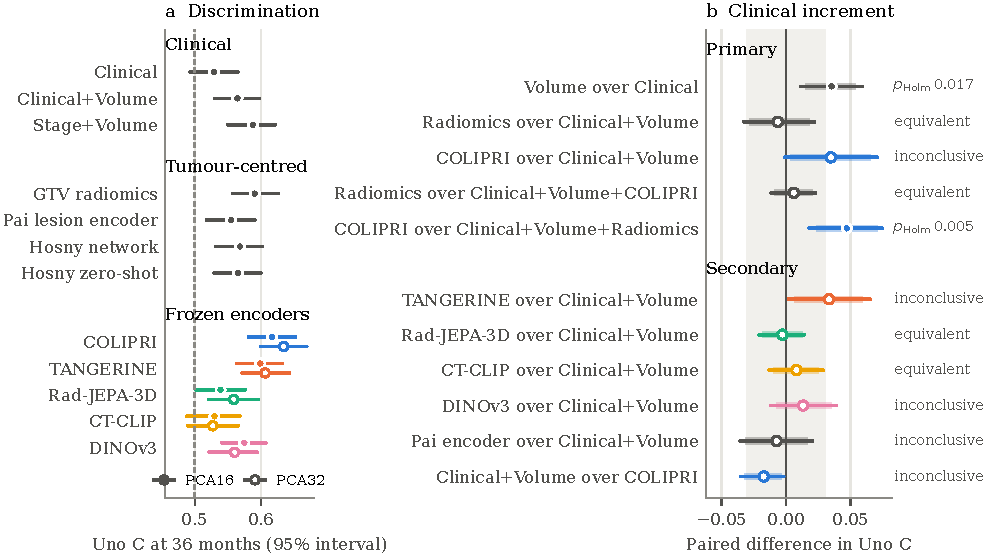
\includegraphics[width=\linewidth]{figures/results_rq1.pdf}
\caption{RQ1: frozen discrimination on LUNG1. (a) Uno C at 36 months with 95\% intervals for the clinical models, the tumour-centred comparators and the frozen encoders with the primary PCA16 linear Cox head (filled markers) and the PCA32 sensitivity head (open markers); the dashed line marks chance. (b) Paired differences between nested clinical models: thin lines, 95\% intervals; thick bands, 90\% intervals; shaded area, the $\pm0.03$ equivalence margin; filled markers, $p_\mathrm{Holm}<0.05$. The verdict on the right is ``equivalent'' when the 90\% interval lies within the margin and ``inconclusive'' when neither a difference nor equivalence was shown.}
\label{fig:rq1}
\end{figure}

No encoder differed from \model{Stage+Volume} or from GTV radiomics after Holm correction. COLIPRI exceeded them by 0.029 ($-0.015$ to 0.071) and 0.026 ($-0.015$ to 0.072), both with $p_\mathrm{Holm}=1.00$; the minimum detectable difference was about 0.06. The largest deficit was CT-CLIP against radiomics, $-0.061$ ($-0.114$ to $-0.009$; $p_\mathrm{Holm}=0.14$). With the 32-component head, a sensitivity analysis, COLIPRI reached 0.634 and exceeded \model{Stage+Volume} by 0.046 ($-0.001$ to 0.093) and radiomics by 0.043 (0.001 to 0.084); neither difference remained significant after Holm correction ($p_\mathrm{Holm}=0.38$ for both), and no other encoder exceeded either baseline. COLIPRI also exceeded the tumour-centred deep models, by 0.062 over the Pai lesion encoder ($p=0.009$, $p_\mathrm{Holm}=0.056$) and by 0.051 over Hosny zero-shot ($p_\mathrm{Holm}=0.14$), without reaching significance after correction.

The contrasts between nested clinical models fall into a primary and a secondary group (Figure~\ref{fig:rq1}b), which differ in the question they address rather than in the encoder. The primary contrasts follow the prespecified sequence of nested models, in which each step adds one block (tumour volume, radiomics, COLIPRI) to the previous model, and answer the main question of which information adds to the clinical covariates. The secondary contrasts lie outside this sequence and check its conclusions: they add each of the other four foundation models or the tumour-centred Pai lesion encoder to \model{Clinical+Volume}, and, in the reverse direction, add the clinical covariates and tumour volume to an image representation alone. The primary contrasts formed one Holm family and each type of secondary contrast its own, so that the supporting comparisons did not dilute the primary ones. In the primary family, tumour volume was the only block that added discrimination to the clinical covariates after correction: \model{Clinical+Volume} exceeded \model{Clinical} by 0.035 (0.011 to 0.059; $p_\mathrm{Holm}=0.017$). Radiomics added nothing to \model{Clinical+Volume} ($-0.006$; 90\% interval $-0.028$ to 0.018, equivalent). COLIPRI added 0.035 ($-0.001$ to 0.070; $p_\mathrm{Holm}=0.18$), a difference smaller than the minimum detectable difference of 0.052, so this contrast is inconclusive rather than negative. Once COLIPRI was in the model, radiomics again added nothing (0.006; 90\% interval $-0.009$ to 0.020, equivalent). Conversely, COLIPRI added to radiomics: \model{Clinical+Volume+Radiomics+COLIPRI} exceeded \model{Clinical+Volume+Radiomics} by 0.047 (0.018 to 0.075; $p_\mathrm{Holm}=0.005$), so the image block added to the radiomic model even though it was not shown to add to \model{Clinical+Volume}.

The secondary contrasts followed the same pattern. TANGERINE over \model{Clinical+Volume} gave 0.033 (0.002 to 0.065; $p_\mathrm{Holm}=0.19$), and DINOv3 0.013 (inconclusive); Rad-JEPA-3D and CT-CLIP were equivalent to adding nothing, and the Pai lesion encoder gave $-0.007$ ($-0.036$ to 0.020; inconclusive). In the reverse direction, adding the clinical covariates to COLIPRI lowered its discrimination by 0.017 ($-0.035$ to $-0.002$; $p_\mathrm{Holm}=0.18$), and left TANGERINE unchanged ($-0.001$, equivalent). The best combined model, \model{Clinical+Volume+Radiomics+COLIPRI}, reached 0.606, below COLIPRI alone.

Thus the frozen global vectors of COLIPRI and TANGERINE contained prognostic information at least comparable to that of stage, tumour volume and radiomics, and largely overlapping with it; none of the encoders was shown to outperform these baselines.


\subsection{RQ2: How do trainable heads, adaptation of the encoder and the training-label budget change survival discrimination?}\label{sec:res-adaptation}

Table~\ref{tab:trainable_results} compares the trainable models with the frozen head of the same representation, all trained on the whole development set and tested on the same patients. The frozen values in the table differ from Figure~\ref{fig:rq1} by at most 0.002, because here the frozen head was refitted with its penalty selected on the same inner folds as the trainable models, so that the two were compared under identical model selection.
\begin{table}[!htbp]
\centering\footnotesize
\caption{Frozen and trainable survival models with all training labels. Mean-fold Uno C at 36 months over the five outer folds; every model was trained on the whole development set of each fold and evaluated on the same test patients. Differences are against the PCA16 frozen head of the same representation, with paired bootstrap intervals (1,000 resamples within folds) and Holm-adjusted $p$ values across 22 comparisons. $^{\dagger}$The adaptation configuration was chosen on these test folds in a preliminary analysis (Section~\ref{sec:res-adaptation}), so these estimates are optimistic. $^{\ddagger}$Training was unstable: the loss spiked during the first epochs and the predicted risks varied little between patients.}
\label{tab:trainable_results}
\begin{tabular}{@{}llrlr@{}}
\toprule
Representation & Model & Uno C & Difference vs PCA16 (95\% interval) & $p_\mathrm{Holm}$ \\
\midrule
COLIPRI & Frozen linear Cox, PCA16 & 0.616 & -- & -- \\
 & Frozen linear Cox, PCA32 & 0.634 & +0.018 (-0.006 to +0.042) & -- \\
 & Multilayer perceptron & 0.621 & +0.005 (-0.016 to +0.027) & 1.000 \\
 & Survival query adapter & 0.615 & -0.001 (-0.025 to +0.024) & 1.000 \\
 & LoRA$^{\dagger}$ & 0.639 & +0.023 (+0.000 to +0.049) & 1.000 \\
 & Partial fine-tuning$^{\dagger}$ & 0.600 & -0.016 (-0.035 to +0.004) & 1.000 \\
\addlinespace
TANGERINE & Frozen linear Cox, PCA16 & 0.600 & -- & -- \\
 & Frozen linear Cox, PCA32 & 0.607 & +0.006 (-0.014 to +0.025) & -- \\
 & Multilayer perceptron & 0.615 & +0.015 (-0.010 to +0.037) & 1.000 \\
 & Survival query adapter & 0.625 & +0.024 (-0.004 to +0.051) & 1.000 \\
 & LoRA$^{\dagger}$ & 0.630 & +0.030 (+0.006 to +0.053) & 0.407 \\
 & Partial fine-tuning$^{\dagger}$ & 0.629 & +0.028 (+0.002 to +0.051) & 0.478 \\
\addlinespace
Rad-JEPA-3D & Frozen linear Cox, PCA16 & 0.539 & -- & -- \\
 & Frozen linear Cox, PCA32 & 0.559 & +0.020 (-0.007 to +0.047) & -- \\
 & Multilayer perceptron & 0.541 & +0.001 (-0.025 to +0.030) & 1.000 \\
 & Survival query adapter & 0.521 & -0.018 (-0.057 to +0.020) & 1.000 \\
 & LoRA & 0.520 & -0.019 (-0.053 to +0.013) & 1.000 \\
 & Partial fine-tuning & 0.540 & +0.001 (-0.029 to +0.029) & 1.000 \\
\addlinespace
CT-CLIP & Frozen linear Cox, PCA16 & 0.530 & -- & -- \\
 & Frozen linear Cox, PCA32 & 0.527 & -0.003 (-0.031 to +0.024) & -- \\
 & Multilayer perceptron & 0.495 & -0.035 (-0.068 to -0.004) & 0.620 \\
 & Survival query adapter & 0.524 & -0.006 (-0.044 to +0.035) & 1.000 \\
 & LoRA$^{\ddagger}$ & 0.500 & -0.030 (-0.082 to +0.024) & 1.000 \\
 & Partial fine-tuning$^{\ddagger}$ & 0.508 & -0.022 (-0.067 to +0.020) & 1.000 \\
\addlinespace
DINOv3 & Frozen linear Cox, PCA16 & 0.575 & -- & -- \\
 & Frozen linear Cox, PCA32 & 0.560 & -0.014 (-0.041 to +0.009) & -- \\
 & Multilayer perceptron & 0.561 & -0.014 (-0.048 to +0.020) & 1.000 \\
 & Survival query adapter & 0.552 & -0.022 (-0.058 to +0.011) & 1.000 \\
 & LoRA & 0.577 & +0.003 (-0.030 to +0.034) & 1.000 \\
 & Partial fine-tuning & 0.582 & +0.008 (-0.016 to +0.033) & 1.000 \\
\addlinespace
Pai lesion encoder & Frozen linear Cox, PCA16 & 0.557 & -- & -- \\
 & Frozen linear Cox, PCA32 & 0.561 & +0.004 (-0.022 to +0.029) & -- \\
 & Multilayer perceptron & 0.588 & +0.031 (+0.005 to +0.056) & 0.407 \\
\addlinespace
Hosny network & Frozen linear Cox, PCA16 & 0.568 & -- & -- \\
 & Frozen linear Cox, PCA32 & 0.554 & -0.014 (-0.041 to +0.015) & -- \\
 & Multilayer perceptron & 0.542 & -0.026 (-0.061 to +0.008) & 1.000 \\
\bottomrule
\end{tabular}
\end{table}


No trainable model differed from the frozen head after Holm correction across the 22 primary comparisons (all $p_\mathrm{Holm}\geq0.41$). The multilayer perceptron changed discrimination by $-0.035$ (CT-CLIP) to $+0.031$ (Pai lesion encoder), and the survival query adapter by $-0.022$ (DINOv3) to $+0.024$ (TANGERINE). The epoch chosen by inner cross-validation was unstable across outer folds, ranging from 2 to 99 for the DINOv3 multilayer perceptron and from 9 to 98 for COLIPRI.

The adaptation configuration (LoRA, learning rate $10^{-3}$; partial fine-tuning, $10^{-4}$; 20 epochs) was fixed a priori, before this analysis, and applied unchanged to all five encoders. Adaptation did not improve on the frozen head: DINOv3 changed by $+0.003$ with LoRA and $+0.008$ with partial fine-tuning, and Rad-JEPA-3D by $-0.019$ and $+0.001$. The largest gains were for the selected encoders, TANGERINE with LoRA ($+0.030$; $+0.006$ to $+0.053$; $p_\mathrm{Holm}=0.41$) and partial fine-tuning ($+0.028$; $p_\mathrm{Holm}=0.48$) and COLIPRI with LoRA ($+0.023$; $+0.000$ to $+0.049$; $p_\mathrm{Holm}=1.00$); these are optimistic and were not significant. For CT-CLIP, the fixed configuration did not train: in every fold, the loss rose from about 5.0 to 6.0--13.4 within three epochs, and with LoRA it then returned to its initial value; and the predicted linear predictor had a within-fold standard deviation of 0.02--0.30, against 0.36--1.1 for the other encoders. The CT-CLIP adaptation results ($-0.030$ and $-0.022$) therefore reflect a failed optimization, not an absence of exploitable information. Doubling head capacity to PCA32 changed the frozen estimates by $-0.014$ to $+0.020$, none significant.

Reducing the number of training patients lowered every model in parallel (Figure~\ref{fig:rq2}). From 100\% to 10\% of the labels (about 333 to 33 patients per fold), COLIPRI fell from 0.617 to 0.550 and TANGERINE from 0.599 to 0.558, while \model{Stage+Volume} fell from 0.588 to 0.537 and radiomics from 0.591 to 0.533. At no budget did any encoder differ from either baseline after Holm correction within the budget (40 comparisons; smallest $p_\mathrm{Holm}=0.058$, for CT-CLIP below radiomics at 25\%). At 10\%, the differences from \model{Stage+Volume} were $+0.013$ ($-0.013$ to $+0.040$) for COLIPRI and $+0.021$ ($-0.003$ to $+0.046$) for TANGERINE.

Neither more flexible heads nor encoder adaptation therefore improved on the frozen linear head, and the frozen representations showed no advantage in label efficiency over the clinical and radiomic baselines.

\begin{figure}[!htbp]
\centering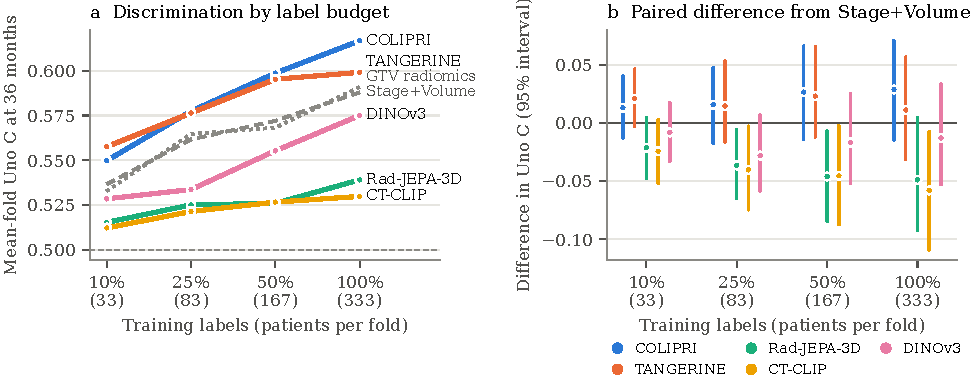
\includegraphics[width=\linewidth]{figures/results_rq2.pdf}
\caption{RQ2: discrimination by training-label budget. (a) Mean-fold Uno C of the frozen PCA16 heads and of the \model{Stage+Volume} (dashed) and radiomic (dotted) baselines, refitted on nested subsets of each development set (ten draws below 100\%) and evaluated on the unchanged test folds. (b) Paired difference of each encoder from \model{Stage+Volume} at each budget, with 95\% intervals (300 resamples). None was significant after Holm correction.}
\label{fig:rq2}
\end{figure}


\subsection{RQ3: How sensitive are the representations and their survival predictions to the tumour?}\label{sec:res-rq3}

The four tumour analyses, described in Section~\ref{sec:perturbation} (Figure~\ref{fig:rq3design}), are summarized in Figure~\ref{fig:rq3}.

\begin{figure}[!t]
\centering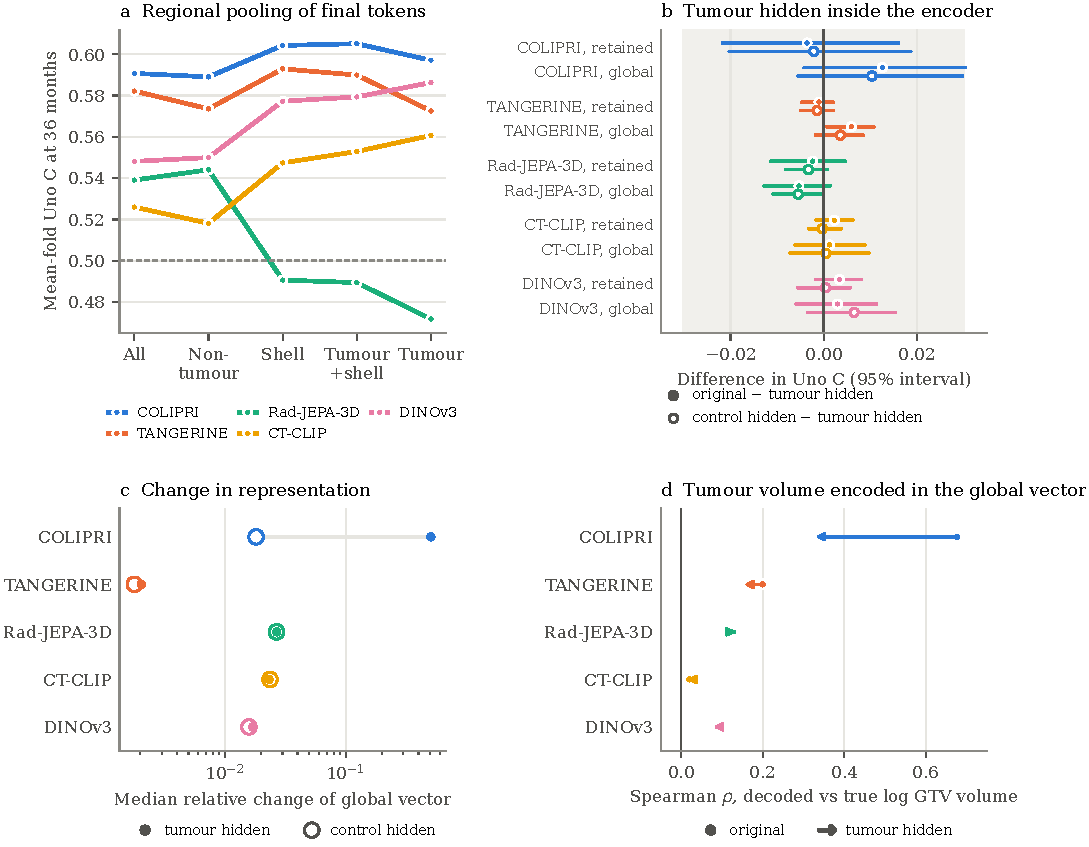
\includegraphics[width=\linewidth]{figures/results_rq3.pdf}
\caption{RQ3: dependence on the tumour. (a) Mean-fold Uno C of the frozen head applied to final tokens pooled over regions defined by the GTV (Section~\ref{sec:perturbation}); the all-token pool is a uniform mean and differs from the encoders' global vectors. (b) Native-token masking in the 403 patients with a matched control: paired differences in Uno C, with retained (mean of tokens visible in every condition) and global vectors; shaded area, $\pm0.03$. Intervals use 300 paired resamples and are not adjusted for multiplicity. (c) Median relative change of the global vector when the tumour or the matched control was hidden (logarithmic scale). (d) Decodability of log GTV volume from the global vector (PCA16 ridge probe), original and with the tumour hidden.}
\label{fig:rq3}
\end{figure}

\paragraph{Regional pooling.} Pooling the final tokens over different regions changed discrimination little except for Rad-JEPA-3D (Figure~\ref{fig:rq3}a). For every encoder, the non-tumour pool was within 0.009 of the all-token pool, because the tumour occupies few token positions. For COLIPRI, the tumour pool differed from the all-token pool by $+0.006$ ($-0.019$ to $+0.031$), and the shell and tumour-plus-shell pools scored highest (0.604 and 0.605). Restricting Rad-JEPA-3D to tumour tokens lowered its discrimination to 0.472, $-0.067$ ($-0.110$ to $-0.025$) relative to all tokens. CT-CLIP and DINOv3 improved numerically with tumour pooling, by $+0.035$ ($-0.015$ to $+0.081$) and $+0.038$ ($-0.005$ to $+0.075$). For TANGERINE and Rad-JEPA-3D, adding the shell to the tumour raised discrimination by about 0.02 (lower bounds $+0.001$ and $+0.004$).

\paragraph{Native-token masking.} Hiding the tumour inside the encoder barely changed discrimination (Figure~\ref{fig:rq3}b). In the 403 patients with a valid control, the original-minus-masked difference on the retained tokens, the primary pooling, ranged from $-0.004$ (COLIPRI; $-0.022$ to $+0.016$) to $+0.003$ (DINOv3), and every interval lay within the equivalence margin. With the global vector, the largest differences were $+0.013$ for COLIPRI ($-0.004$ to $+0.030$), $+0.006$ for TANGERINE ($+0.001$ to $+0.011$) and $-0.005$ for Rad-JEPA-3D ($-0.013$ to $+0.001$). The differences between the control-hidden and tumour-hidden conditions were of the same size, so hiding the tumour was no more harmful than hiding any comparable region.

The representations themselves responded differently (Figure~\ref{fig:rq3}c). Hiding the tumour changed the COLIPRI global vector by a median of 51\%, against 2\% for the matched control. For the other four encoders, the tumour and the control changed the global vector by the same amount (0.2\% to 2.7\%), so these vectors were insensitive to the tumour specifically.

\paragraph{Fixed head.} When the head fitted on original embeddings was applied unchanged to the masked ones, COLIPRI fell from 0.623 to 0.610 with the global vector (difference $+0.013$; $-0.002$ to $+0.029$), with a similar difference for the retained tokens ($+0.012$; $-0.003$ to $+0.028$), whereas hiding the control changed it by less than 0.001. The rank correlation between original and masked risk scores was 0.92 for COLIPRI and at least 0.996 for every other encoder. The fitted COLIPRI model therefore used some tumour-derived information, but losing it cost little discrimination.

\paragraph{Clinical-variable probing.} The embeddings explain why (Figure~\ref{fig:rq3}d). The COLIPRI global vector encoded tumour volume (Spearman $\rho=0.68$) and T3--T4 category (AUC 0.70); hiding the tumour reduced these to 0.32 (difference 0.36; 0.28 to 0.44) and 0.55 (difference 0.15; 0.09 to 0.19). Age ($\rho=0.70$ to 0.69) and stage III (AUC 0.70 to 0.72) were unaffected. The other encoders encoded tumour volume weakly ($\rho\leq0.20$) but encoded sex strongly (AUC 0.78 to 0.999); TANGERINE also encoded age ($\rho=0.71$) and stage III (AUC 0.75), all unchanged by masking. Histology was not decodable (AUC 0.42--0.64).

Only COLIPRI was sensitive to the tumour, and it encoded tumour size, the block that added most to the clinical covariates in RQ1. Yet hiding the tumour halved the decodable volume and lowered discrimination by at most 0.013, indicating that most of the prognostic information in these representations was carried by the rest of the scan.


\subsection{RQ4: Do discrimination, incremental clinical value and calibration transfer to an external cohort?}\label{sec:res-rq4}

\begin{table}[!htbp]
\centering\footnotesize
\caption{External evaluation in NSCLC-Radiogenomics (143 patients, 33 deaths by 36 months). Models were fitted on all 416 LUNG1 patients and frozen before external outcomes were read. Internal and external values are Uno C at 36 months; internal is the mean-fold LUNG1 estimate. External intervals come from 2,000 patient resamples and condition on the frozen models. $p_\mathrm{Holm}$ tests external Uno C against 0.5, Holm-adjusted across all models. Calibration slope: coefficient of the linear predictor in an external Cox regression (1 is ideal). Predicted: mean predicted 36-month mortality with the LUNG1 baseline hazard; observed Kaplan--Meier mortality was 0.25. The Hosny zero-shot score has no baseline hazard. $^{\ddagger}$Exploratory: fixed LoRA configuration, trained on all LUNG1 patients after the external cohort had been examined; it was chosen on the COLIPRI and TANGERINE test folds. Internal values are the LoRA estimates of Table~\ref{tab:trainable_results}. $^{\dagger}$Unadjusted $p$ against 0.5; the exploratory LoRA analysis was not corrected for multiplicity. $^{\S}$Training did not converge; predicted risks were almost constant.}
\label{tab:external}
\begin{tabular}{@{}lrlrrr@{}}
\toprule
Model & Internal & External (95\% interval) & $p_\mathrm{Holm}$ & Slope & Predicted \\
\midrule
\multicolumn{6}{@{}l}{\textit{Clinical and radiomic}}\\
\model{Clinical} & 0.529 & 0.595 (0.493 to 0.698) & 0.402 & 1.73 & 0.66 \\
\model{Clinical+Volume} & 0.565 & 0.646 (0.547 to 0.749) & 0.067 & 1.76 & 0.63 \\
\model{Stage+Volume} & 0.588 & 0.605 (0.508 to 0.702) & 0.367 & 3.24 & 0.67 \\
GTV radiomics & 0.591 & 0.617 (0.508 to 0.723) & 0.299 & 0.45 & 0.62 \\
\multicolumn{6}{@{}l}{\textit{Clinical and image}}\\
\model{Clinical+Volume+COLIPRI} & 0.599 & 0.653 (0.557 to 0.748) & 0.027 & 1.84 & 0.64 \\
\model{Clinical+Volume+Radiomics+COLIPRI} & 0.606 & 0.652 (0.555 to 0.751) & 0.040 & 0.92 & 0.67 \\
\multicolumn{6}{@{}l}{\textit{Frozen image representations}}\\
COLIPRI & 0.617 & 0.627 (0.540 to 0.719) & 0.077 & 1.90 & 0.65 \\
TANGERINE & 0.599 & 0.649 (0.550 to 0.741) & 0.041 & 0.62 & 0.50 \\
Rad-JEPA-3D & 0.539 & 0.530 (0.436 to 0.627) & 1.000 & 0.05 & 0.84 \\
CT-CLIP & 0.530 & 0.482 (0.388 to 0.581) & 1.000 & -0.57 & 0.64 \\
DINOv3 & 0.575 & 0.643 (0.556 to 0.730) & 0.021 & 1.26 & 0.85 \\
Pai lesion encoder & 0.555 & 0.547 (0.446 to 0.646) & 1.000 & 0.48 & 0.66 \\
Hosny zero-shot & 0.566 & 0.540 (0.432 to 0.643) & 1.000 & 0.13 & -- \\
\multicolumn{6}{@{}l}{\textit{Exploratory LoRA adaptation}$^{\ddagger}$}\\
COLIPRI, LoRA & 0.639 & 0.687 (0.606 to 0.768) & $<$0.001$^{\dagger}$ & 0.79 & 0.53 \\
TANGERINE, LoRA & 0.630 & 0.633 (0.536 to 0.728) & 0.007$^{\dagger}$ & 0.57 & 0.61 \\
Rad-JEPA-3D, LoRA & 0.520 & 0.442 (0.329 to 0.556) & 0.311$^{\dagger}$ & -0.28 & 0.81 \\
CT-CLIP, LoRA$^{\S}$ & 0.500 & 0.505 (0.405 to 0.606) & 0.924$^{\dagger}$ & 5.52 & 0.68 \\
DINOv3, LoRA & 0.577 & 0.623 (0.528 to 0.721) & 0.012$^{\dagger}$ & 0.22 & 0.48 \\
\bottomrule
\end{tabular}
\end{table}

Externally, discrimination was maintained or higher for COLIPRI, TANGERINE and DINOv3 and lost for Rad-JEPA-3D, CT-CLIP and the tumour-centred deep models (Table~\ref{tab:external}; Figure~\ref{fig:rq4}a). TANGERINE reached 0.649 (0.550 to 0.741), DINOv3 0.643 and COLIPRI 0.627, compared with 0.646 for \model{Clinical+Volume} and 0.605 for \model{Stage+Volume}. After Holm correction, TANGERINE ($p_\mathrm{Holm}=0.041$) and DINOv3 (0.021) exceeded chance, as did \model{Clinical+Volume+COLIPRI}, \model{Clinical+Volume+DINOv3} and both \model{Clinical+Volume+Radiomics+Image} models, whereas COLIPRI (0.077), \model{Clinical+Volume} (0.067) and \model{Stage+Volume} (0.37) did not. Rad-JEPA-3D (0.530), CT-CLIP (0.482), the Pai lesion encoder (0.547) and Hosny zero-shot (0.540) were at chance. The ranking of the 22 models was largely preserved (Spearman $\rho=0.67$, $p<0.001$).

None of the four primary contrasts was significant or equivalent. COLIPRI exceeded \model{Stage+Volume} by 0.021 ($-0.068$ to $0.126$), the Pai lesion encoder by 0.080 ($-0.031$ to $0.195$) and Hosny zero-shot by 0.087 ($-0.046$ to $0.231$), and \model{Clinical+Volume+COLIPRI} exceeded \model{Clinical+Volume} by 0.007 ($-0.052$ to $0.071$); all $p_\mathrm{Holm}\geq0.67$. The minimum detectable differences were 0.088 for the clinical increment and 0.13 to 0.20 for the others, several times the size of the internal differences, so these contrasts are uninformative.

Absolute risks did not transport (Figure~\ref{fig:rq4}b). Observed 36-month mortality was 25\%, whereas mean predicted mortality ranged from 37\% to 85\% and was at least 58\% for every model except TANGERINE (50\%) and \model{Clinical+Volume+TANGERINE} (37\%). Calibration slopes ranged from $-0.57$ (CT-CLIP) to 3.24 (\model{Stage+Volume}); for COLIPRI it was 1.90, indicating that its predicted risks were not spread widely enough for the external population.

In the exploratory external LoRA analysis, adaptation improved external discrimination only for COLIPRI, which reached 0.687 (0.606 to 0.768), 0.060 above its frozen head (0.004 to 0.120). For the other encoders, LoRA was at or below the frozen head: TANGERINE $-0.016$ ($-0.107$ to $+0.073$), DINOv3 $-0.019$ ($-0.101$ to $+0.067$) and Rad-JEPA-3D $-0.088$ ($-0.172$ to $-0.011$), with Rad-JEPA-3D falling below chance (0.442). As internally, CT-CLIP did not train and its predicted risks were almost constant. Intervals are not adjusted for multiplicity, and the COLIPRI and TANGERINE models were trained in FP16 rather than BF16. Because the configuration was chosen on LUNG1 test folds and the analysis was added after the external cohort had been examined, the single COLIPRI gain is a hypothesis for independent testing, not evidence that adaptation transfers.

Risk ordering by the stronger frozen encoders therefore transported to a population with a different stage, treatment and scanner mix, whereas their incremental value over clinical models could not be resolved with 33 external events, and their absolute risks required recalibration.

\begin{figure}[!htbp]
\centering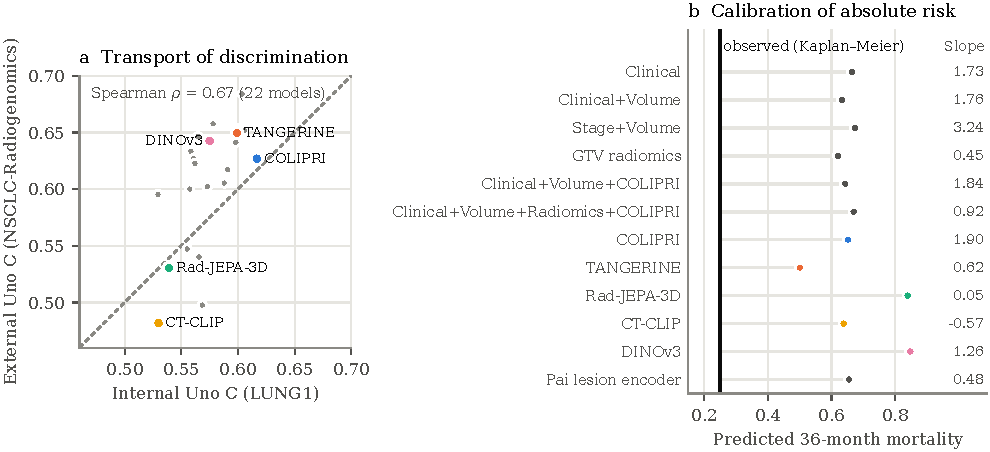
\includegraphics[width=\linewidth]{figures/results_rq4.pdf}
\caption{RQ4: external evaluation in NSCLC-Radiogenomics (143 patients). (a) Internal (LUNG1 mean-fold) against external Uno C at 36 months for the 22 frozen models; coloured points are the frozen encoders, grey points the clinical, radiomic, tumour-centred and combined models; the dashed line is identity. (b) Mean predicted 36-month mortality with the LUNG1 baseline hazard against the observed Kaplan--Meier mortality (vertical line); the column on the right gives the external calibration slope.}
\label{fig:rq4}
\end{figure}

\section{Discussion}\label{sec:discussion}

\subsection{Principal findings}
This study compared five foundation models with clinical, radiomic and tumour-centred models for overall survival in NSCLC, within one protocol and on the same patients and folds. Four findings emerge.

First, frozen whole-volume representations contained prognostic information, but not more than the established predictors could be shown to provide. COLIPRI had the highest internal discrimination and exceeded \model{Stage+Volume} and radiomics by 0.026 to 0.029 in point estimate with the primary head and by 0.043 to 0.046 with PCA32, but no difference was significant after correction. Among the blocks added to the clinical covariates, only tumour volume improved discrimination significantly; no encoder was shown to add to \model{Clinical+Volume}. COLIPRI did add to the model that already contained radiomics, by 0.047, so it carried information that radiomics did not. Second, more training did not help: neither trainable heads nor LoRA or partial fine-tuning improved on a linear Cox head on the frozen embedding, and the encoders were no more label-efficient than the baselines. Third, the survival predictions depended little on the tumour. Hiding the tumour inside the encoder changed discrimination by at most 0.013, although for COLIPRI it changed the embedding substantially and halved the decodable tumour volume. Fourth, risk ordering transported to an external surgical cohort for TANGERINE, DINOv3 and COLIPRI, whereas their incremental value over clinical models could not be resolved and their absolute risks were poorly calibrated.

\subsection{Comparison with previous work}
The absence of a benefit from adaptation agrees with the two studies that compared frozen and adapted encoders for prognosis: frozen lesion-encoder features outperformed fine-tuned variants,\cite{pai2024} and LoRA and full fine-tuning of CT-CLIP gave no advantage over the frozen encoder.\cite{allgower2026} Our results extend this to five encoders, to label budgets from 10\% to 100\% and to a paired statistical comparison. They also suggest one reason: in about 330 patients per development set, the trainable models selected very different numbers of epochs across folds, an indication that the signal available for optimization is weak relative to its noise. The fixed adaptation configuration did not train at all for CT-CLIP, so a configuration transferred between encoders is not a neutral choice.

The competitiveness of radiomics and of simple clinical predictors is consistent with recent benchmarks on LUNG1, in which handcrafted features matched foundation-model features\cite{neukirch2026} and frozen lesion-centred embeddings discriminated only modestly.\cite{aerts2025tib} Those benchmarks used binary two-year endpoints and frozen heads; with a censoring-aware endpoint, trainable and adapted models, and paired equivalence testing, the conclusion is the same. The best internal estimates (0.59 to 0.63) also lay within the range reported for prognostic models in this cohort (Section~\ref{sec:cohorts}).\cite{aerts2014}

Our tumour analyses reach a different conclusion from earlier work on tumour dependence. In the network of Hosny and colleagues, removing the context around the tumour reduced discrimination,\cite{hosny2018} and occlusion saliency has localized to the lesion for some encoders.\cite{aerts2025tib} Those analyses studied tumour-centred models or perturbed the input image. Intervening inside frozen whole-volume encoders, with a matched control, showed that their survival predictions were largely carried by the rest of the scan.

\subsection{What the representations encode}
The probing and masking results suggest how a whole-volume embedding can predict survival without relying on the tumour. COLIPRI encoded tumour size, and it was the only encoder whose embedding and fitted model responded to hiding the tumour; yet losing half of the decodable volume cost little discrimination, so the remaining information was largely redundant with it. The other encoders encoded tumour volume weakly but sex strongly and, for TANGERINE and DINOv3, age, consistent with representations dominated by patient-level anatomy rather than by the lesion. This may explain why the same encoders transported externally. In an early-stage surgical cohort, many deaths are likely not caused by the cancer, and representations of age and general health could rank patients as well as stage and volume, which vary little in that population; this was the expectation recorded in the external protocol. TANGERINE and DINOv3, which encoded age and sex but little tumour information, transported best. These explanations are post hoc. Decodability shows that a variable is encoded, not that the survival prediction uses it, and the analyses do not identify a biological mechanism.

\subsection{Limits of the available input}
Discrimination converged across model families. Internally, the clinical covariates, tumour volume, radiomics, the tumour-centred networks and the five encoders all lay between about 0.53 and 0.64, and neither trainable heads, encoder adaptation nor additional training patients moved the leading encoders beyond this range; externally, the three stronger encoders lay within about 0.02 of \model{Clinical+Volume}. When representations that differ this much in origin and capacity reach a similar level, the limit is more plausibly set by what the input contains than by how it is modelled. Overall survival depends on factors that pretreatment CT and the recorded clinical variables reflect only indirectly, such as performance status, comorbidity, lung function and the treatment actually delivered; neither cohort records performance status or comorbidity, and LUNG1 does not record the treatment received. The encoders appear to recover part of this information through proxies: they encoded age and sex and drew on the patient rather than on the tumour, which may explain why they matched, but did not exceed, the clinical models. Two considerations temper this interpretation. Recording these variables is not sufficient by itself: a model developed at the institution that provided LUNG1, which included performance status, lung function and delivered dose, reached a concordance of 0.62,\cite{oberije2015} close to the level observed here, so part of this limit may reflect the intrinsic unpredictability of overall survival, which includes deaths unrelated to the cancer and events that depend on care after baseline. And with a few hundred patients, differences below the minimum detectable difference cannot be excluded, so the convergence holds at the resolution of this study and does not show that larger encoders, or adaptation tuned for each encoder, could not help. Further progress therefore seems more likely to come from cohorts that record the patient and the treatment alongside the image, and from larger samples, than from larger or more extensively adapted encoders.

\subsection{Implications}
For clinical use, the results do not support replacing or augmenting clinical predictors with frozen foundation-model embeddings: no incremental value over the clinical covariates and tumour volume was demonstrated internally or externally, and absolute risks would require recalibration in every new population. For research, they argue for three practices. Foundation-model survival studies should report paired comparisons against a parsimonious clinical model and against radiomics, with equivalence margins and minimum detectable differences, because differences of a few hundredths are the scale of interest and are below the detection limit of cohorts of a few hundred patients. Adaptation choices should be selected without the test folds, and their stability checked per encoder. Finally, claims that a model ``looks at the tumour'' need interventions with matched controls, because a change in the representation need not change the prediction.

\section{Limitations}\label{sec:limitations}
The main limitation of this study is its size. The differences between models were a few hundredths of Uno C, often smaller than either cohort could reliably detect: the minimum detectable difference, the smallest difference detectable with 80\% power, was about 0.02 to 0.07 internally and, with 33 deaths by 36 months, 0.09 to 0.20 externally. Most contrasts were therefore inconclusive rather than negative, and the external analysis can neither establish nor exclude incremental value. The uncertainty we report is also likely to be underestimated. All internal analyses used a single partition into five outer folds, and the bootstrap intervals condition on the fitted models and on that partition, so they do not include the variability from refitting on different patients or from a different fold assignment.

A second group of limitations concerns how the development cohort was used. LUNG1 served for every internal analysis. The PCA32 head was added after the PCA16 comparisons, the external LoRA analysis after the external cohort had been examined, and the label-budget, masking and probing analyses are exploratory, with intervals not adjusted for multiplicity. The adaptation itself was limited in scope. A single configuration was transferred to all encoders without tuning; it failed for CT-CLIP, which was moreover adapted at its visual projection rather than at an encoder block, so its results do not show what a tuned configuration would achieve, and full fine-tuning was not examined. The clinical reference was restricted to the covariates shared by both cohorts, and neither cohort records performance status or comorbidity, so the incremental value of the encoders was assessed against a weaker clinical model than is available in practice, and the interpretation that the available input limits discrimination could not be tested directly.

The comparisons between pipelines have their own limits. Each encoder kept its published preprocessing and global pooling, so the differences combine pretraining, preprocessing, field of view and pooling, and cannot be attributed to the pretraining objective; the tumour-centred comparators, in turn, received the tumour location that the whole-volume encoders did not. The comparators were not all exact reproductions: the Hosny network, reimplemented from the published weights, did not fully reproduce the published patient-level predictions on LUNG1, and the radiomic model is a practical baseline rather than the original LUNG1 signature. The tumour interventions also require caution. Hidden tokens contain the tissue around the tumour within their footprint, the masked inputs lie outside the distribution on which the encoders were trained, and regional pooling locates information by token position rather than by tissue of origin, because tokens exchange information inside the encoder. Robustness to masking therefore does not show that the tumour carries no prognostic information.

Finally, the external cohort differs from LUNG1 in stage, treatment, scanners and the source of TNM, which was pathological rather than clinical. Survival was measured from the CT date because treatment dates were unavailable, and the segmentation labels required manual verification. In LUNG1, the legacy codes T5 and N4 were merged by an analytic convention whose clinical meaning is uncertain. Some encoders were pretrained on public chest CT collections, and the overlap between their pretraining data and either cohort has not been fully audited.

\section{Conclusions}\label{sec:conclusions}
Frozen CT foundation models captured prognostic information in NSCLC comparable to, but not demonstrably greater than, stage, tumour volume and radiomics; trainable heads and encoder adaptation did not improve on a linear head; and the predictions depended little on the tumour itself. Their risk ordering transported to an external cohort, but their incremental clinical value remains unresolved and their absolute risks require recalibration. Because discrimination converged across clinical, radiomic and foundation models, the input available in public cohorts, rather than the choice of model, appears to limit prognostic performance. Larger cohorts that record the patient and the treatment, prespecified adaptation choices and evaluation of incremental value over clinical models are needed before these representations can be considered for prognostic use.

\section*{Declarations}
\gap{Authors must supply affiliations, contributions, funding, conflicts of interest, and the applicable ethics and data-use statements. Public dataset availability does not itself establish an ethics exemption.}
\noindent\textbf{Code availability.} Analysis code, experimental protocols and aggregate result summaries are available at \url{https://github.com/nico9902/ct-fm-prognostic-transferability}. Software dependencies are documented in the repository requirements files. Imaging data and pretrained model weights must be obtained separately from their respective sources.
\noindent\textbf{Draft AI-assistance disclosure for author review.} An AI coding assistant assisted with manuscript organization, prose drafting, reference discovery, and generation of tables and figures from existing aggregate analysis outputs. Authors must verify the text, references, analyses, and disclosure against the selected journal's policy before submission.
\bibliographystyle{vancouver}
\bibliography{references}
\clearpage
% \appendix
% \section{Preliminary fixed-epoch analysis}\label{app:fixed}
% Before the adaptation configuration was fixed, LoRA and partial fine-tuning of COLIPRI and TANGERINE were examined over the same learning rates for 5 or 20 epochs, giving 24 configurations. Each fit used the whole development set (approximately 332 patients) and was evaluated at the final epoch on the same test folds, so no data were held out for choosing among configurations. This appendix reports all of them without selection.

% All 24 configurations completed five folds (Figure~\ref{fig:sweep}; Table~\ref{tab:phase3}). For both encoders and both methods, mean-fold Uno C increased with the learning rate and with 20 rather than 5 epochs. At the lowest learning rates, performance was close to chance (0.485--0.529). At the highest learning rate with 20 epochs, LoRA reached 0.639 for COLIPRI and 0.630 for TANGERINE, and partial fine-tuning reached 0.600 and 0.629. These settings lay at the upper edge of the grid, so higher learning rates or longer training were not examined. Performance varied between folds: for the best LoRA configuration, fold-level Uno C ranged from 0.571 to 0.719 for COLIPRI and from 0.536 to 0.695 for TANGERINE.

% The frozen reference head, fitted on the same development sets and evaluated on the same test folds, reached 0.617 for COLIPRI and 0.599 for TANGERINE. In point estimate, the best LoRA configuration exceeded the frozen head by 0.022 for COLIPRI and 0.031 for TANGERINE; the best partial fine-tuning configuration exceeded it by 0.030 for TANGERINE but remained 0.017 below it for COLIPRI. Because these configurations were identified from test-fold results, this difference is not an unbiased estimate of the benefit of adaptation, and no hypothesis test is attached to it. The configuration with the highest mean Uno C for both encoders (LoRA $10^{-3}$, partial fine-tuning $10^{-4}$, 20 epochs) was then fixed for all five encoders (Section~\ref{sec:selected}); for COLIPRI and TANGERINE, the main-text adaptation results are these fits and are therefore optimistic.

% \begin{figure}[!htbp]
% \centering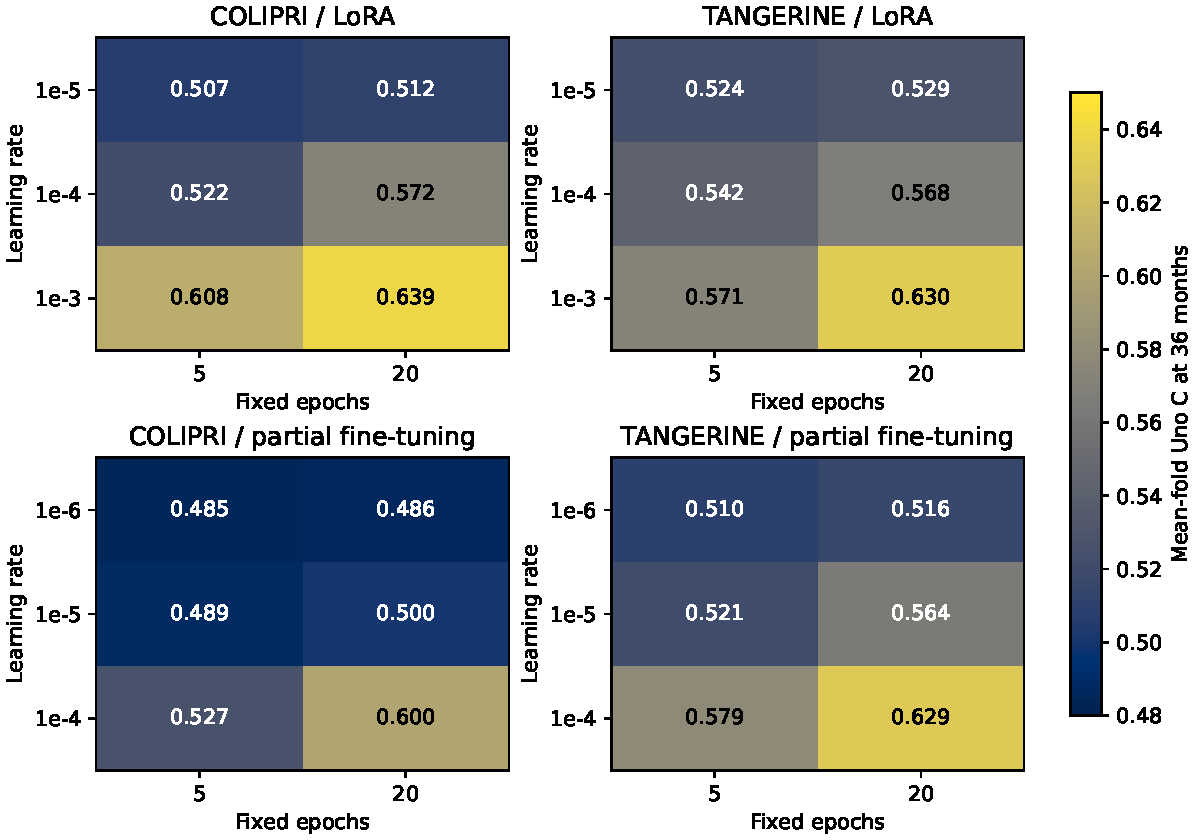
\includegraphics[width=\linewidth]{figures/phase3_sweep.pdf}
% \caption{Preliminary fixed-epoch analysis of encoder adaptation for COLIPRI and TANGERINE. Each cell is mean Uno C through 36 months across the five outer folds, evaluated at the final epoch. The colour scale is descriptive; cells are not independent evaluations of an optimally selected method.}\label{fig:sweep}
% \end{figure}
% \begin{longtable}{llrrr}
\caption{All 24 configurations of the preliminary fixed-epoch analysis (Appendix~\ref{app:fixed}). Each value is mean-fold Uno C at 36 months over five completed folds, evaluated at the final epoch.}\label{tab:phase3}\\
\toprule Method & Learning rate & Epochs & COLIPRI & TANGERINE \\ \midrule
\endfirsthead
\toprule Method & Learning rate & Epochs & COLIPRI & TANGERINE \\ \midrule
\endhead
LoRA & 1e-5 & 5 & 0.5069 & 0.5238 \\
LoRA & 1e-5 & 20 & 0.5124 & 0.5285 \\
LoRA & 1e-4 & 5 & 0.5224 & 0.5420 \\
LoRA & 1e-4 & 20 & 0.5721 & 0.5680 \\
LoRA & 1e-3 & 5 & 0.6081 & 0.5715 \\
LoRA & 1e-3 & 20 & 0.6393 & 0.6301 \\
Partial fine-tuning & 1e-6 & 5 & 0.4852 & 0.5098 \\
Partial fine-tuning & 1e-6 & 20 & 0.4864 & 0.5163 \\
Partial fine-tuning & 1e-5 & 5 & 0.4885 & 0.5207 \\
Partial fine-tuning & 1e-5 & 20 & 0.5004 & 0.5642 \\
Partial fine-tuning & 1e-4 & 5 & 0.5266 & 0.5787 \\
Partial fine-tuning & 1e-4 & 20 & 0.6005 & 0.6289 \\
\bottomrule
\end{longtable}

\end{document}
